\chapter[Separation Theorems in the Plane]{Separation Theorems \\in the Plane}
\vspace{6.5cm}
\chaptermark{Separation Theorems in the Plane}


There are several difficult questions concerning the topology of the plane that arise quite naturally in the study of analysis. The answers to these questions seem geometrically quite obvious but turn out to be surprisingly hard to prove. They include the \index{jordan curve theorem@Jordan curve theorem}, the Brouwer theorem on \index{Invariance of domain}, and the classical theorem that the \index{Winding number} of a simple \index{closed topologist's sine curve@Closed topologist's sine curve} closed curve is zero or \(\pm  1\) . We prove them in this chapter as consequences \index{Fundamental group!of double torus}of our study of covering spaces and the \index{Double torus!fundamental group}fundamental group

\section*{§ 61 The Jordan Separation Theorem}

We consider first one of the classical theorems of mathematics, the \index{jordan curve theorem@Jordan curve theorem}Jordan curve theorem. It states a fact that is geometrically quite believable, the fact that a \index{Simple closed curve!separates \({S}^{2}\)}\index{simple closed curve@Simple closed curve}simple closed curve in the plane always \index{separates a space@Separates a space} separates the plane into two pieces, its ``inside'' and its ``outside.'' It was originally conjectured in 1892 by Camille Jordan, and several incorrect proofs were published, including one by Jordan himself. Eventually, a correct proof was provided by Oswald Veblen, in 1905. The early proofs were complicated, but over the years, simpler proofs have been found. If one uses the tools of modern algebraic topology, singular homology theory in particular, the proof is quite straightforward. The proof we give here is the simplest one we know that uses only results from the theory of covering spaces and the fundamental group.

Our proof of the Jordan curve theorem divides into three parts. The first, which we call the \index{jordan separation theorem@Jordan separation theorem}, states that a simple closed curve in the plane separates it into at least two components. The second says that an arc in the plane does not separate the plane. And the third, the Jordan curve theorem proper, says that a simple closed curve \(C\) in the plane separates it into precisely two components, of which \(C\) is the common boundary. The first of these theorems will be treated in this section.

In dealing with separation theorems, it will often be convenient to formulate them as separation theorems for subsets of \({S}^{2}\) rather than \({\mathbb{R}}^{2}\) . The separation theorems for \({\mathbb{R}}^{2}\) will follow. The connection between the two sets of theorems is provided by the following lemma.

Recall that if \(b\) is any point of \({S}^{2}\) , there is a homeomorphism \(h\) of \({S}^{2} - b\) with \({\mathbb{R}}^{2}\) ; one simply takes a rotation of \({S}^{2}\) that carries \(b\) to the north pole, and follows it by stereographic projection.

\begin{lemma}
	Let \(C\) be a compact subspace of \({S}^{2}\) ; let \(b\) be a point of \({S}^{2} - C\) ; and let \(h\) be a homeomorphism of \({S}^{2} - b\) with \({\mathbb{R}}^{2}\) . Suppose \(U\) is a component of \({S}^{2} - C\) . If \(U\) does not contain \(b\) , then \(h( U)\) is a bounded component of \({\mathbb{R}}^{2} - h( C)\) . If \(U\) contains \(b\) , then \(h( {U - b})\) is the unbounded component of \({\mathbb{R}}^{2} - h( C)\) .
\end{lemma}

In particular, if \({S}^{2} - C\) has \(n\) components, then \({\mathbb{R}}^{2} - h( C)\) has \(n\) components.

\begin{proof}
	We show first that if \(U\) is a component of \({S}^{2} - C\) , then \(U - b\) is connected. This result is trivial if \(b \notin  U\) , so suppose that \(b \in  U\) and suppose the sets \(A\) and \(B\) form a separation of \(U - b\) . Choose a neighborhood \(W\) of \(b\) disjoint from \(C\) such that \(W\) is homeomorphic to an open ball of \({\mathbb{R}}^{2}\) . Since \(W\) is connected, it is contained in \(U\) ; since \(W - b\) is connected, it is contained entirely in \(A\) or in \(B\) . Say \(W - b \subset  A\) . Then \(b\) is not a limit point of \(B\) , for \(W\) is a neighborhood of \(b\) disjoint from \(B\) . It follows that the sets \(A \cup  \{ b\}\) and \(B\) form a separation of \(U\) , contrary to hypothesis.
Let \(\{  {U}_{\alpha }\}\) be the set of components of \({S}^{2} - C\) ; let \({V}_{\alpha } = h( {{U}_{\alpha } - b})\) . Because \({S}^{2} - C\) is locally connected, the sets \({U}_{\alpha }\) are connected, disjoint, open subsets of \({S}^{2}\) . Therefore, the sets \({V}_{\alpha }\) are connected, disjoint, open subsets of \({\mathbb{R}}^{2} - h( C)\) , so the sets \({V}_{\alpha }\) are the components of \({\mathbb{R}}^{2} - h( C)\) .

Now the homeomorphism \(h\) of \({S}^{2} - b\) with \({\mathbb{R}}^{2}\) can be extended to a homeomorphism \(H\) of \({S}^{2}\) with the one-point compactification \({\mathbb{R}}^{2} \cup  \{ \infty \}\) of \({\mathbb{R}}^{2}\) , merely by setting \(H( b)  = \infty\) . If \({U}_{\beta }\) is the component of \({S}^{2} - C\) containing \(b\) , then \(H( {U}_{\beta })\) is a neighborhood of \(\infty\) in \({\mathbb{R}}^{2} \cup  \{ \infty \}\) . Therefore \({V}_{\beta }\) is unbounded; since its complement \({\mathbb{R}}^{2} - {V}_{\beta }\) is compact, all the other components of \({\mathbb{R}}^{2} - h( C)\) are bounded. See Figure 61.1.
\end{proof}
\begin{lemma}[Null \index{free homotopy of loops@Free homotopy of loops}homotopy lemma]
	Let \(a\) and \(b\) be points of \({S}^{2}\) . Let \(A\) be a compact space, and let

\[
f : A \rightarrow  {S}^{2} - a - b
\]

be a continuous map. If \(a\) and \(b\) lie in the same component of \({S}^{2} - f( A)\) , then \(f\) is nulhomotopic.

\begin{center}
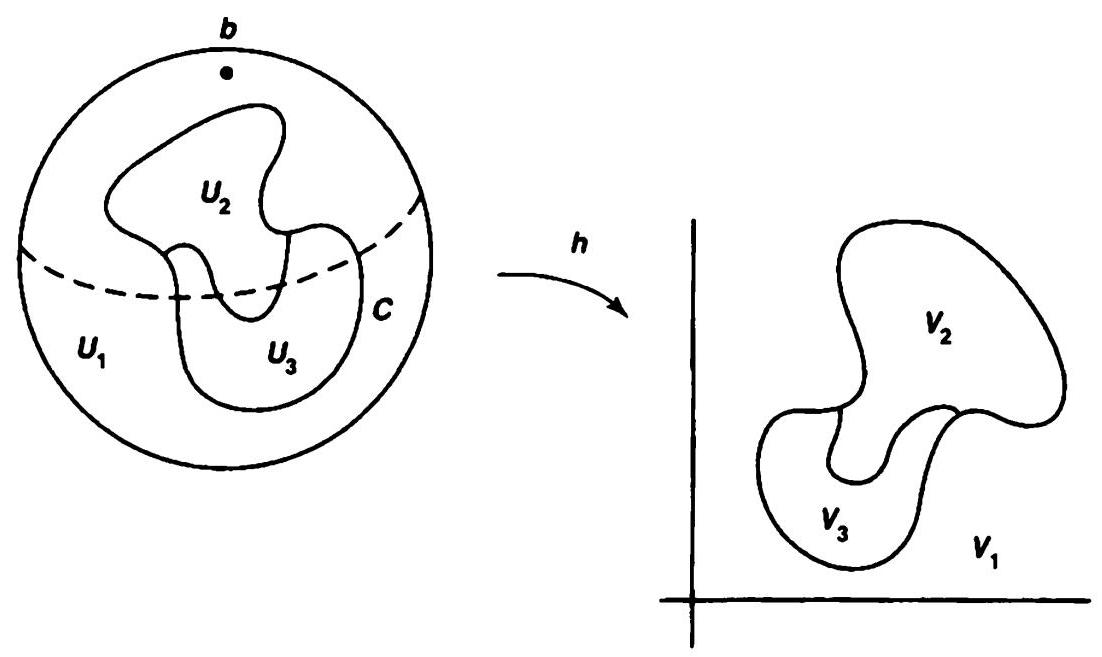
\includegraphics[width=1.0\textwidth]{images/61.1.jpg}
\end{center}
\hspace*{3em} 

Figure 61.1
\end{lemma}

\begin{proof}
	One can replace \({S}^{2}\) by the one-point compactification \({\mathbb{R}}^{2} \cup  \{ \infty \}\) of \({\mathbb{R}}^{2}\) , letting \(a\) and \(b\) correspond to the points0and \(\infty\) . Then our lemma reduces to the following: Let \(A\) be a compact space and let \(g : A \rightarrow  {\mathbb{R}}^{2} - 0\) be a continuous map. If0lies in the unbounded component of \({\mathbb{R}}^{2} - g( A)\) , then \(g\) is nulhomotopic.
This statement is easy to prove. Choose a ball \(B\) centered at the orgin, of sufficiently large radius that it contains the set \(g( A)\) . Choose a point \(p\) of \({\mathbb{R}}^{2}\) lying outside \(B\) . Then0and \(p\) both lie in the unbounded component of \({\mathbb{R}}^{2} - g( A)\) .

Because \({\mathbb{R}}^{2}\) is locally path connected, so is the open set \({\mathbb{R}}^{2} - g( A)\) . Therefore, the components and path components of \({\mathbb{R}}^{2} - g( A)\) are the same. Hence we can choose a path \(\alpha\) in \({\mathbb{R}}^{2} - g( A)\) from 0 to \(p\) . We define a homotopy \(G : A \times  I \rightarrow  {\mathbb{R}}^{2} -\) 0 by the equation

\[
G( {x,t})  = g( x)  - \alpha ( t) ;
\]

it is pictured in Figure 61.2. The homotopy \(G\) is a homotopy between the map \(g\) and the map \(k\) defined by \(k( x)  = g( x)  - p\) . Note that \(G( {x,t})  \neq  0\) because the path \(\alpha\) does not intersect the set \(g( A)\) .

Now we define a homotopy \(H : A \times  I \rightarrow  {\mathbb{R}}^{2} - 0\) by the equation

\[
H( {x,t})  = \operatorname{tg}( x)  - p.
\]

It is a homotopy between the map \(k\) and a constant map. Note that \(H( {x,t})  \neq  0\) because \({tg}( x)\) lies inside the ball \(B\) and \(p\) does not.

Thus we have proved that \(g\) is nulhomotopic.

Now we prove the \index{jordan separation theorem@Jordan separation theorem}Jordan separation theorem. In \index{Nonseparation theorem: arc in \({S}^{2}\)!general}general, if \(X\) is a connected space and \(A \subset  X\) , we say that \(A\) separates \(X\) if \(X - A\) is not connected; if \(X - A\) has \(n\) components, we say that \(A\) \index{separates a space@Separates a space}separates \(X\) \index{Separates a space!into \(n\) components}into n components.

\begin{center}
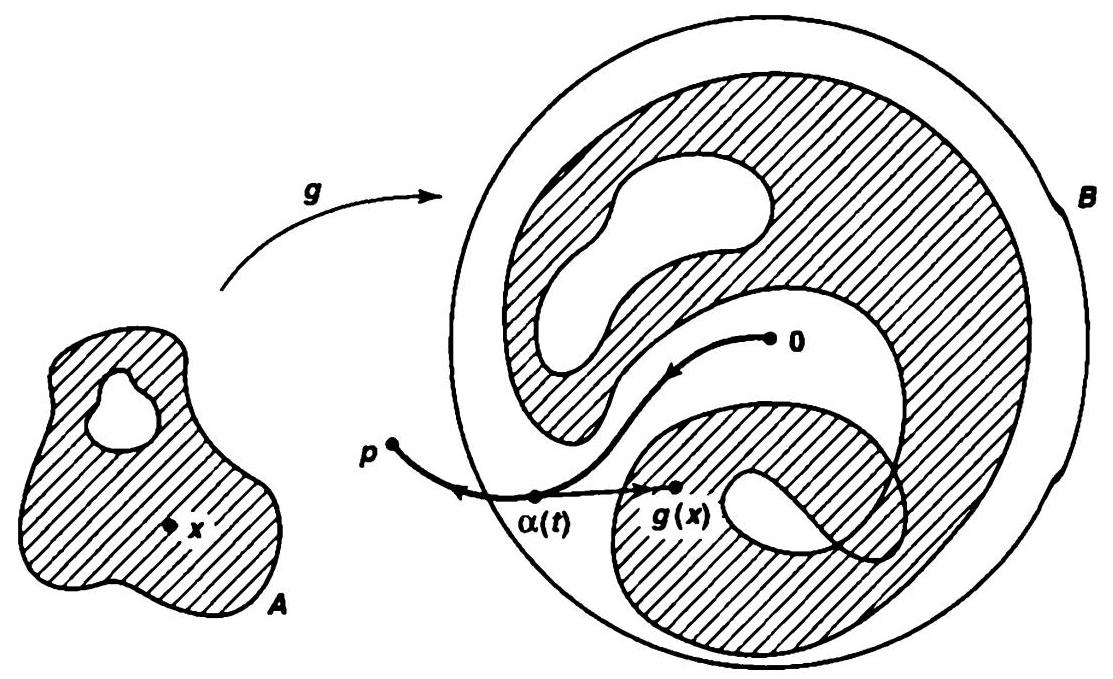
\includegraphics[width=1.0\textwidth]{images/61.2.jpg}
\end{center}
\hspace*{3em} 

Figure 61.2

An arc \(A\) is a space homeomorphic to the unit interval \([  {0,1}]\) . The end points of \(A\) are the two points \(p\) and \(q\) of \(A\) such that \(A - p\) and \(A - q\) are connected; the other points of \(A\) are called \index{interior point: of an arc@Interior point: of an arc} interior points of \(A\) .

A simple closed curve is a space homeomorphic to the unit circle \({S}^{1}\) .
\end{proof}
\begin{theorem}[The Jordan separation theorem]
	Let \(C\) be a \index{Separation theorem: closed topologist's sine curve in \({S}^{2}\)!simple closed curve in \({S}^{2}\)}simple closed curve in \({S}^{2}\) . Then \(C\) \index{Closed topologist's sine curve!separates \({S}^{2}\)}separates \({S}^{2}\) .
\end{theorem}

\begin{proof}
	Because \({S}^{2} - C\) is locally path connected, its components and path components are the same. We assume that \({S}^{2} - C\) is path connected and derive a contradiction.
Let us write \(C\) as the union of two arcs \({A}_{1}\) and \({A}_{2}\) that intersect only in their end points \(a\) and \(b\) . Let \(X\) denote the space \({S}^{2} - a - b\) . Let \(U\) be the open set \({S}^{2} - {A}_{1}\) of \(X\) , and let \(V\) be the open set \({S}^{2} - {A}_{2}\) . Then \(X\) is the union of the sets \(U\) and \(V\) , and

\[
U \cap  V = {S}^{2} - ( {{A}_{1} \cup  {A}_{2}})  = {S}^{2} - C,
\]

which by hypothesis is path connected Thus the hypotheses of Theorem 59.1 are satisfied.

Let \({x}_{0}\) be a point of \(U \cap  V\) . We will show that the inclusions

\[
i : ( {U,{x}_{0}})  \rightarrow  ( {X,{x}_{0}}) \;\text{ and }\;j : ( {V,{x}_{0}})  \rightarrow  ( {X,{x}_{0}})
\]

induce trivial homomorphisms of the fundamental groups involved. It then follows from Theorem 59.1 that the group \({\pi }_{1}( {X,{x}_{0}})\) is trivial. But \(X = {S}^{2} - a - b\) , which is homeomorphic to the punctured plane \({\mathbb{R}}^{2} - \mathbf{0}\) , so its fundamental group is not trivial.

Let us prove that \({i}_{ * }\) is the trivial homomorphism; given a loop \(f : I \rightarrow  U\) based at \({x}_{0}\) , we show that \({i}_{ * }( [  f]  )\) is trivial. For this purpose, let \(p : I \rightarrow  {S}^{1}\) be the standard loop generating \({\pi }_{1}( {{S}^{1},{b}_{0}})\) . The map \(f : I \rightarrow  U\) induces a continuous map \(h : {S}^{1} \rightarrow\)  \(U\) such that \(h \circ  p = f\) . See Figure 61.3.

Consider the map \(i \circ  h.{S}^{1} \rightarrow  {S}^{2} - a - b\) . By hypothesis, the set \(i( {h( {S}^{1}) })  = h( {S}^{1})\) does not intersect the connected set \({A}_{1}\) containing \(a\) and \(b\) . Therefore, \(a\) and \(b\) lie in the same component of \({S}^{2} - i( {h( {S}^{1}) })\) . By the preceding lemma, the map \(i \circ  h\) is \index{Nulhomotopic map!induces trivial homomorphism}nulhomotopic. It follows from Lemma 55.3 that \({( i \circ  h) }_{ * }\) is the trivial homomorphism of fundamental groups. But

\[
{( i \circ  h) }_{ * }( [  p]  )  = [  {i \circ  h \circ  p}] = [  {i \circ  f}] = {i}_{ * }( [  f]  ) .
\]

Therefore, \({i}_{ * }( [  f]  )\) is trivial, as desired.

\begin{center}
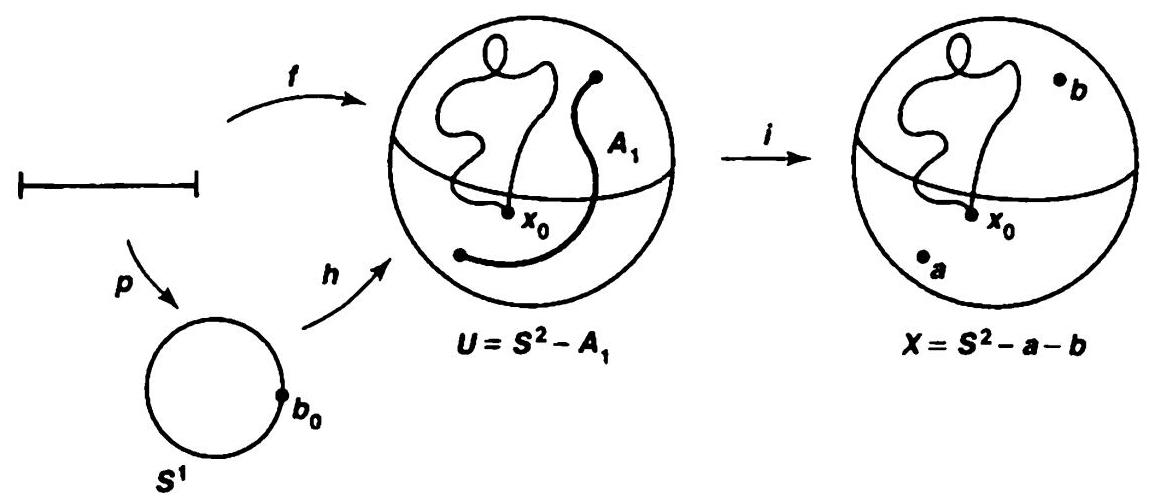
\includegraphics[width=1.0\textwidth]{images/61.3.jpg}
\end{center}
\hspace*{3em} 

Figure 61.3

Let us examine the preceding proof. What facts did we use about the simple closed curve \(C\) ? All we actually needed was the fact that \(C\) could be written as the union of the two closed connected sets \({A}_{1}\) and \({A}_{2}\) , whose intersection consisted of the two points \(a\) and \(b\) . This remark leads to the following \index{Separation theorem: closed topologist's sine curve in \({S}^{2}\)!general}\index{general separation theorem@General separation theorem}generalized version of the separation theorem, which will be useful later.
\end{proof}
\begin{theorem}[A \index{General separation theorem}]
	Let \({A}_{1}\) and \({A}_{2}\) be closed connected subsets of \({S}^{2}\) whose intersection consists of precisely two points a and \(b\) . Then the set \(C = {A}_{1} \cup  {A}_{2}\) separates \({S}^{2}\) .
\end{theorem}

\begin{proof}
	We must show first that \(C\) cannot equal all of \({S}^{2}\) . That fact was obvious in the earlier proof. In the present case, we can see that \(C \neq  {S}^{2}\) because \({S}^{2} - a - b\) is connected and \(C - a - b\) is not. (The sets \({A}_{i} - a - b\) form a separation of \(C - a - b\) .)
The remainder of the proof is a copy of the proof of the preceding theorem.
\end{proof}
\section*{Exercises}
\begin{enumerate}[itemsep=0.4em, parsep=0pt, topsep=0pt, partopsep=0pt, leftmargin=*, label=\arabic*., ref=\arabic*]
\item Give examples to show that a simple closed curve in the \index{double torus@Double torus} torus may or may not separate the torus.
\item Let \(A\) be the subset of \({\mathbb{R}}^{2}\) consisting of the union of the topologist's sine curve and the broken-line path from \(( {0, - 1})\) to \(( {0, - 2})\) to \(( {1, - 2})\) to \(( {1,\sin 1})\) . See Figure 61.4. We call \(A\) the \index{closed topologist's sine curve@Closed topologist's sine curve}closed topologist's sine curve. Show that if \(C\) is a subspace of \({S}^{2}\) homeomorphic to the closed topologist's sine curve, then \(C\) separates \({S}^{2}\) . \begin{center} 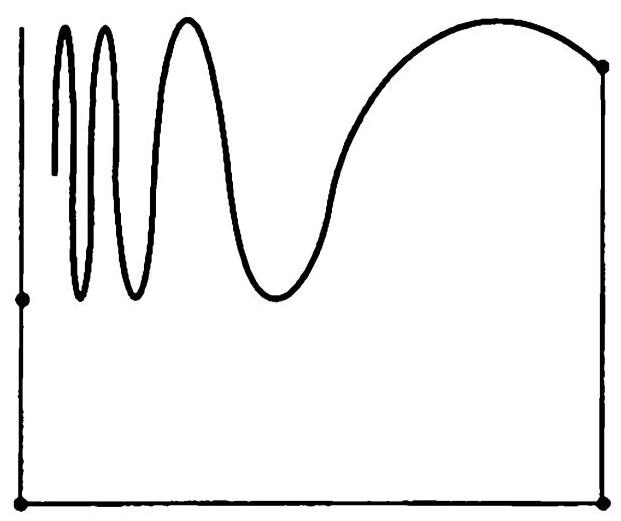
\includegraphics[width=0.5\textwidth]{images/61.4.jpg} \end{center} \hspace*{3em} Figure 61.4
\end{enumerate}
\section*{*§ 62 Invariance of Domain \protect\sectionDagger}

One of the theorems of topology that is truly fundamental, because it expresses an intrinsic property of euclidean space, is the theorem on ``\index{invariance of domain@Invariance of domain}invariance of domain,'' proved by L. E. J. Brouwer in 1912. It states that for any open set \(U\) of \({\mathbb{R}}^{n}\) and any continuous injective mapping \(f : U \rightarrow  {\mathbb{R}}^{n}\) , the image set \(f( U)\) is open in \({\mathbb{R}}^{n}\) and the inverse function is continuous. (The Inverse Function Theorem of analysis derives this result under the additional hypothesis that the map \(f\) is continuously differentiable with nonsingular Jacobian matrix.) We shall prove this theorem in the case \(n = 2\) .

\begin{lemma}[\index{homotopy extension lemma@Homotopy extension lemma}]
	Let \(X\) be a space such that \(X \times  I\) is normal. Let \(A\) be a closed subspace of \(X\) , and let \(f : A \rightarrow  Y\) be a continuous map, where \(Y\) is an open subspace of \({\mathbb{R}}^{n}\) . If \(f\) is nulhomotopic, then \(f\) may be extended to a continuous map \(g : X \rightarrow  Y\) that is also nulhomotopic.
\end{lemma}

\begin{proof}
	Let \(F : A \times  I \rightarrow  Y\) be a homotopy between \(f\) and a constant map. Then \(F( {a,0})  = f( a)\) and \(F( {a,1})  = {y}_{0}\) for all \(a\) . Extend \(F\) to the space \(X \times  1\) by setting \(F( {x,1})  = {y}_{0}\) for \(x \in  X\) Then \(F\) is a continuous map of the closed subspace \((A \times\)  \(I) \cup  ( {X \times  1})\) of \(X \times  I\) into \({\mathbb{R}}^{n}\) ; by the Tietze extension theorem, it may be extended to a continuous map \(G : X \times  I \rightarrow  {\mathbb{R}}^{n}\) .
\customfootnote{${}^{\dagger}$ In this section, we use the Tietze extension theorem ( \S 35).}

Now the map \(x \rightarrow  G( {x,0})\) is an extension of \(f\) , but it maps \(X\) into \({\mathbb{R}}^{n}\) rather than into the subspace \(Y\) To obtain our desired map, we proceed as follows: Let \(U\) be the open subset \(U = {G}^{-1}( Y)\) of \(X \times  I\) . Then \(U\) contains \(( {A \times  I})  \cup  ( {X \times  1})\) . See Figure 62.1. Since \(I\) is compact, the tube lemma implies that there is an open set \(W\) of \(X\) containing \(A\) such that \(W \times  I \subset  U\) . Now the space \(X\) is itself normal, being homeomorphic to the closed subspace \(X \times  0\) of \(X \times  I\) . Therefore, we may choose a continuous function \(\phi  : X \rightarrow  [  {0,1}]\) such that \(\phi ( x)  = 0\) for \(x \in  A\) and \(\phi ( x)  = 1\) for \(x \in  X - W\) . The map \(x \rightarrow  x \times  \phi ( x)\) carries \(X\) into the subspace \(( {W \times  I})  \cup  ( {X \times  1})\) of \(X \times  I\) , which lies in \(U\) . Then the continuous map \(g( x)  = G( {x,\phi ( x) })\) carries \(X\) into \(Y\) . And for \(x \in  A\) , we have \(\phi ( x)  = 0\) , so that \(g( x)  = G( {x,0})  = f( x)\) . Thus \(g\) is the desired extension of \(f\) . The map \(H : X \times  I \rightarrow  Y\) given by

\[
H( {x,t})  = G( {x,( {1 - t}) \phi ( x)  + t})
\]

is a homotopy between \(g\) and a constant map.

\begin{center}
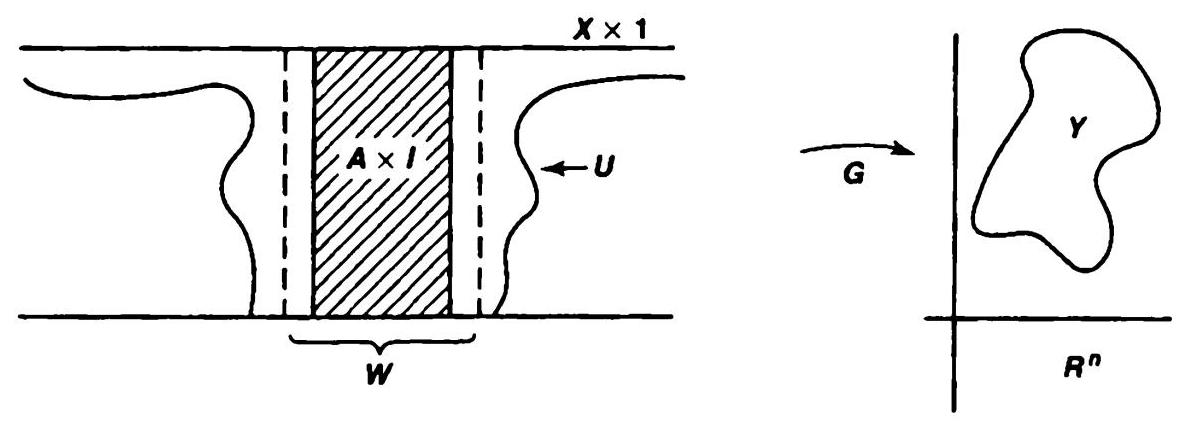
\includegraphics[width=1.0\textwidth]{images/62.1.jpg}
\end{center}
\hspace*{3em} 

Figure 62.1

The following lemma is a partial converse to the nulhomotopy lemma of the preceding section.
\end{proof}
\begin{lemma}[\index{borsuk lemma@Borsuk lemma}]
	Let \(a\) and \(b\) be points of \({S}^{2}\) . Let \(A\) be a compact space, and let \(f : A \rightarrow  {S}^{2} - a - b\) be a continuous injective map. If \(f\) is nulhomotopic, then \(a\) and \(b\) lie in the same component of \({S}^{2} - f( A)\) .
\end{lemma}

\begin{proof}
	Because \(A\) is compact and \({S}^{2}\) is Hausdorff, \(f( A)\) is a compact subspace of \({S}^{2}\) that is homeomorphic to \(A\) . Because \(f\) is nulhomotopic, so is the inclusion mapping of \(f( A)\) into \({S}^{2} - a - b\) . Hence it suffices to prove the lemma in the special case where \(f\) is simply an inclusion map. Furthermore, we can replace \({S}^{2}\) by \({\mathbb{R}}^{2} \cup  \{ \infty \}\) , letting \(a\) correspond to 0, and \(b\) to \(\infty\) . Then our lemma reduces to the following statement:
Let \(A\) be a compact subspace of \({\mathbb{R}}^{2} - \mathbf{0}\) . If the inclusion \(j : A \rightarrow  {\mathbb{R}}^{2} - \mathbf{0}\) is nulhomotopic, then0lies in the unbounded component of \({\mathbb{R}}^{2} - A\) .

This we now prove. Let \(C\) be the component of \({\mathbb{R}}^{2} - A\) containing 0; we suppose \(C\) is bounded and derive a contradiction. Let \(D\) be the union of the other components of \({\mathbb{R}}^{2} - A\) , including the unbounded component. Then \(C\) and \(D\) are disjoint open sets of \({\mathbb{R}}^{2}\) , and \({\mathbb{R}}^{2} - A = C \cup  D\) . See Figure 62.2.

We define a continuous map \(h : {\mathbb{R}}^{2} \rightarrow  {\mathbb{R}}^{2} - \mathbf{0}\) that equals the identity outside \(C\) .

Begin with the inclusion map \(j : A \rightarrow  {\mathbb{R}}^{2} - \mathbf{0}\) . Since \(j\) is by hypothesis nulho-motopic, the preceding lemma implies that \(j\) can be extended to a continuous map \(k\) of \(C \cup  A\) into \({\mathbb{R}}^{2} - \mathbf{0}\) . Then \(k\) equals the identity at points of \(A\) . Extend \(k\) to a map \(h : {\mathbb{R}}^{2} \rightarrow  {\mathbb{R}}^{2} - \mathbf{0}\) by setting \(h( x)  = x\) for \(x \in  D \cup  A\) , then \(h\) is continuous by the pasting lemma.

Now we derive a contradiction. Let \(B\) be the closed ball in \({\mathbb{R}}^{2}\) of radius \(M\) centered at the origin, where \(M\) is so large that Int \(B\) contains \(C \cup  A\) . (Here, we use the fact that \(C\) is bounded.) If we restrict \(h\) to \(B\) , we obtain a map \(g : B \rightarrow  {\mathbb{R}}^{2} - 0\) such that \(g( x)  = x\) for \(x \in  \operatorname{Bd}B\) . If we follow \(g\) by the standard retraction \(x \rightarrow  {Mx}/\parallel x\parallel\) of \({\mathbb{R}}^{2} - 0\) onto Bd \(B\) , we obtain a retraction of \(B\) onto Bd \(B\) . Such a retraction does not exist.

\begin{center}
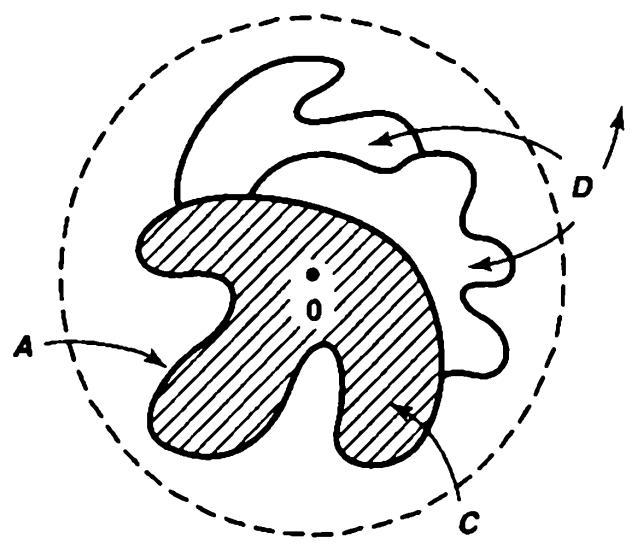
\includegraphics[width=0.5\textwidth]{images/62.2.jpg}
\end{center}
\hspace*{3em} 

Figure 62.2
\end{proof}
\begin{theorem}[Invariance of domain]
	If \(U\) is an open subset of \({\mathbb{R}}^{2}\) and \(f : U \rightarrow\)  \({\mathbb{R}}^{2}\) is continuous and injective, then \(f( U)\) is open in \({\mathbb{R}}^{2}\) and the inverse function \({f}^{-1} : f( U)  \rightarrow  U\) is continuous.
\end{theorem}

\begin{proof}
	As usual, we can replace \({\mathbb{R}}^{2}\) by \({S}^{2}\) . We show that if \(U\) is an open subset of \({\mathbb{R}}^{2}\) and \(f : U \rightarrow  {S}^{2}\) is continuous and injective, then \(f( U)\) is open in \({S}^{2}\) and the inverse function is continuous.
Step 1. We show that if \(B\) is any closed ball in \({\mathbb{R}}^{2}\) contained in \(U\) , then \(f( B)\) does not separate \({S}^{2}\) .

Let \(a\) and \(b\) be two points of \({S}^{2} - f( B)\) . Because the identity map \(i : B \rightarrow  B\) is nulhomotopic, the map \(h : B \rightarrow  {S}^{2} - a - b\) obtained by restricting \(f\) is nulhomotopic. The Borsuk lemma then implies that \(a\) and \(b\) lie in the same component of \({S}^{2} - h( B)  =\)  \({S}^{2} - f( B)\) .

Step 2. We show that if \(B\) is any closed ball of \({\mathbb{R}}^{2}\) lying in \(U\) , then \(f( {\operatorname{Int}B})\) is open in \({S}^{2}\) .

The space \(C = f( {\operatorname{Bd}B})\) is a simple closed curve in \({S}^{2}\) , so it separates \({S}^{2}\) . Let \(V\) be the component of \({S}^{2} - C\) that contains the connected set \(f( {\operatorname{Int}B})\) , and let \(W\) be the union of the others. Because \({S}^{2}\) is locally connected, \(V\) and \(W\) are open in \({S}^{2}\) . We show \(V = f( {\operatorname{Int}B})\) , and we are through.

We suppose \(a\) is a point of \(V\) that is not in \(f( {\operatorname{Int}B})\) and derive a contradiction. Let \(b\) be a point of \(W\) . Since the set \(D = f( B)\) does not separate \({S}^{2}\) , the set \({S}^{2} - D\) is a connected set containing \(a\) and \(b\) . This set is contained in \({S}^{2} - C\) (since \(D \supset  C\) ); it follows that \(a\) and \(b\) lie in the same component of \({S}^{2} - C\) , contrary to construction. See Figure 62.3.

\begin{center}
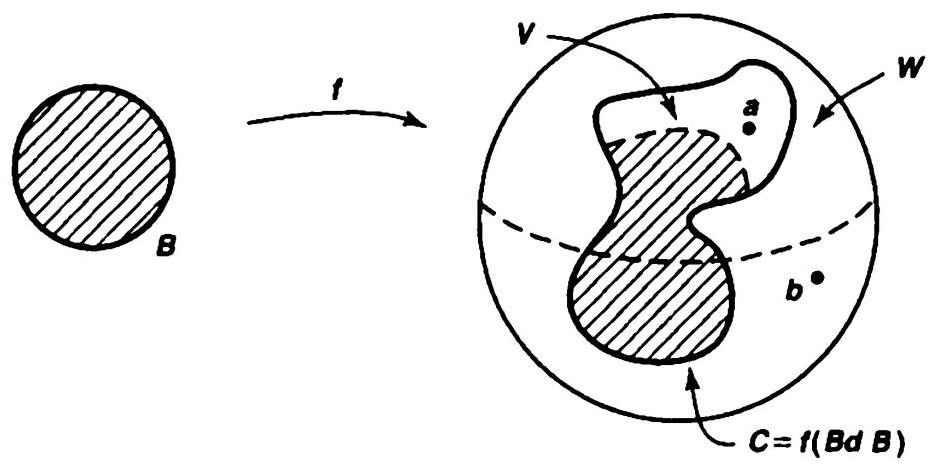
\includegraphics[width=0.8\textwidth]{images/62.3.jpg}
\end{center}
\hspace*{3em} 

Figure 62.3

Step 3. We prove the theorem. Since, for any ball \(B\) contained in \(U\) , the set \(f( {\text{ Int }B})\) is open in \({S}^{2}\) , the map \(f : U \rightarrow  {S}^{2}\) is an open map. It follows that \(f( U)\) is open in \({S}^{2}\) and \({f}^{-1}\) is continuous.
\end{proof}
\section*{Exercises}
\begin{enumerate}[itemsep=0.4em, parsep=0pt, topsep=0pt, partopsep=0pt, leftmargin=*, label=\arabic*., ref=\arabic*]
\item Give an example to show that the conclusion of the Borsuk lemma need not hold if \(f\) is not injective.
\item Let \(A\) be a compact contractible subspace of \({S}^{2}\) . Show that \(A\) does not separate \({S}^{2}\) .
\item Let \(X\) be a space such that \(X \times  I\) is normal. Let \(A\) be a closed subspace of \(X\) ; let \(f : A \rightarrow  Y\) be a continuous map, where \(Y\) is an open subspace of \({\mathbb{R}}^{n}\) . If \(f\) is homotopic to a map that is extendable to a continuous map \(h : X \rightarrow  Y\) , then \(f\) itself is extendable to a continuous map \(g : X \rightarrow  Y\) , such that \(g \simeq  h\) .
\item Let \(C\) be a simple closed curve in \({\mathbb{R}}^{2} - 0\) ; let \(j : C \rightarrow  {\mathbb{R}}^{2} - 0\) be the inclusion mapping. Show that \({j}_{ * }\) is trivial if 0 lies in the unbounded component of \({\mathbb{R}}^{2} - C\) , and is nontrivial otherwise. (In fact, \({j}_{ * }\) is an isomorphism in the latter case, as we shall prove in  \S 65.)
\item Theorem. Let \(U\) be a simply connected open set in \({\mathbb{R}}^{2}\) . If \(C\) is a simple closed curve lying in \(U\) , then each bounded component of \({\mathbb{R}}^{2} - C\) also lies in \(U\) . (This condition actually characterizes the simply connected open sets of \({\mathbb{R}}^{2}\) . See \cite{Rudin1987}. The space \({\mathbb{R}}^{2} - C\) has, of course, only one bounded component, as we shall prove in the next section.)
\item Suppose you are given that there is no retraction of \({B}^{n}\) onto \({S}^{n - 1}\) .
  \begin{enumerate}[itemsep=0.2em, parsep=0pt, topsep=0pt, partopsep=0pt, leftmargin=*, label=(\alph*), align=left]
  \item Show the Borsuk lemma holds for \({S}^{n}\) .
  \item Show that no compact contractible subspace of \({S}^{n}\) separates \({S}^{n}\) .
  \item Suppose you are given also that any subspace of \({S}^{n}\) homeomorphic to \({S}^{n - 1}\) separates \({S}^{n}\) . Prove the invariance of domain theorem in dimension \(n\) .
  \end{enumerate}
\end{enumerate}
\section*{§ 63 The Jordan Curve Theorem}

The special case of the Seifert-van Kampen theorem that we used in proving the Jordan separation theorem tells us something about the fundamental group of the space \(X =\)  \(U \cup  V\) in the case where the intersection \(U \cap  V\) is path connected. In the next theorem, we examine what happens when \(U \cap  V\) is not path connected. This result will enable us to complete the proof of the Jordan curve theorem.

\begin{theorem}
	Let \(X\) be the union of two open sets \(U\) and \(V\) , such that \(U \cap  V\) can be written as the union of two disjoint open sets \(A\) and \(B\) . Assume that there is a path \(\alpha\) in \(U\) from a point \(a\) of \(A\) to a point \(b\) of \(B\) , and that there is a path \(\beta\) in \(V\) from \(b\) to \(a\) . Let \(f\) be the loop \(f = \alpha  * \beta\) .

(a) The path-homotopy class \([  f]\) generates an infinite cyclic subgroup of \({\pi }_{1}( {X,a})\) .

*(b) If \({\pi }_{1}( {X,a})\) is itself infinite cyclic, it is generated by \([  f]  {.}^{\dagger}\)

(c) Assume there is a path \(\gamma\) in \(U\) from a to the point \({a}^{\prime }\) of \(A\) , and that there is a path \(\delta\) in \(V\) from \({a}^{\prime }\) to \(a\) . Let \(g\) be the loop \(g = \gamma  * \delta\) . Then the subgroups of \({\pi }_{1}( {X,a})\) generated by \([  f]\) and \([  g]\) intersect in the identity element alone.
\end{theorem}

\begin{proof}
	The proof is in many ways an imitation of the proof in  \S 54 that the fundamental group of the circle is infinite cyclic. As in that proof, the crucial step is to find an appropriate covering space \(E\) for the space \(X\) .
Step 1. (Construction of \(E\) ). We construct \(E\) by pasting together copies of the subspaces \(U\) and \(V\) . Let us take countably many copies of \(U\) and countably many copies of \(V\) , all disjoint, say

\[
U \times  ( {2n}) \;\text{ and }\;V \times  ( {{2n} + 1})
\]

for all \(n \in  \mathbb{Z}\) , where \(\mathbb{Z}\) denotes the integers. Let \(Y\) denote the union of these spaces; \(Y\) is a subspace of \(X \times  \mathbb{Z}\) . Now we form a new space \(E\) as a quotient space of \(Y\) by identifying the points

\[
x \times  ( {2n}) \;\text{ and }\;x \times  ( {{2n} - 1}) \;\text{ for }x \in  A
\]

\customfootnote{${}^{\dagger}$ This result uses Theorem 54.6, and will be used only when we deal with \index{Simple closed curve!winding number}winding numbers in \S 65.}

and by identifying the points

\[
x \times  ( {2n}) \;\text{ and }\;x \times  ( {{2n} + 1}) \;\text{ for }x \in  B.
\]

Let \(\pi  : Y \rightarrow  E\) be the quotient map.

Now the map \(\rho  : Y \rightarrow  X\) defined by \(\rho ( {x \times  m})  = x\) induces a map \(p : E \rightarrow  X\) ; the map \(p\) is continuous because \(E\) has the quotient topology. The map \(p\) is also surjective. We shall show that \(p\) is a covernng map. See Figure 63.1.

First let us show that the map \(\pi\) is an open map. Since \(Y\) is the union of the disjoint open sets \(\{ U \times  ( {2n}) \}\) and \(\{ V \times  ( {{2n} + 1}) \}\) , it will suffice to show that \(\pi  \mid  ( {U \times  {2n}})\) and \(\pi  \mid  ( {V \times  ( {{2n} + 1}) })\) are open maps. And this is easy. Take an open set in \(U \times  {2n}\) , for example; it will be of the form \(W \times  {2n}\) , where \(W\) is open in \(U\) . Then

\[
{\pi }^{-1}( {\pi ( {W \times  {2n}}) })  = [  {W \times  {2n}}] \cup  [  {( {W \cap  B})  \times  ( {{2n} + 1}) }]
\]

\[
\cup  [  {( {W \cap  A})  \times  ( {{2n} - 1}) }]  \text{ , }
\]

which is the union of three open sets of \(Y\) and hence open in \(Y\) . By definition of the quotient topology, \(\pi ( {W \times  {2n}})\) is open in \(E\) , as desired.

Now we prove that \(p\) is a covering map; we show that the open sets \(U\) and \(V\) are evenly covered by \(p\) . Consider \(U\) , for example. The set \({p}^{-1}( U)\) is the union of the disjoint sets \(\pi ( {U \times  {2n}})\) for \(n \in  \mathbb{Z}\) . Each of these sets is open in \(E\) because \(\pi\) is an open map. Let \({\pi }_{2n}\) denote the restriction of \(\pi\) to the open set \(U \times  {2n}\) , mapping it onto \(\pi ( {U \times  {2n}})\) . It is a homeomorphism because it is bijective, continuous, and open. Then when restricted to \(\pi ( {U \times  {2n}})\) , the map \(p\) is just the composite of the two homeomorphisms

\[
\pi ( {U \times  {2n}}) \xrightarrow[]{{\pi }_{2n}^{-1}}U \times  {2n}\overset{\rho }{ \rightarrow  }U
\]

and is thus a homeomorphism. Therefore, \(p \mid  \pi ( {U \times  {2n}})\) maps this set homeomorphi-cally onto \(U\) , as desired.

Step 2. Now we define a family of liftings of the loop \(f = \alpha  * \beta\) .

For each integer \(n\) , let \({e}_{n}\) be the point \(\pi ( {a \times  {2n}})\) of \(E\) . Then the points \({e}_{n}\) are distinct, and they constitute the set \({p}^{-1}( a)\) . We define a lifting \({\widetilde{f}}_{n}\) of \(f\) that begins at \({e}_{n}\) and ends at \({e}_{n + 1}\) .

Since \(\alpha\) and \(\beta\) are paths in \(U\) and \(V\) , respectively, we can define

\[
\begin{aligned}  & {\bar{\alpha }}_{n}( s)  = \pi ( {\alpha ( s)  \times  {2n}}) , \\  & {\widetilde{\beta }}_{n}( s)  = \pi ( {\beta ( s)  \times  ( {{2n} + 1}) }) ; \end{aligned}
\]

then \({\widetilde{\alpha }}_{n}\) and \({\widetilde{\beta }}_{n}\) are liftings of \(\alpha\) and \(\beta\) , respectively. (The case \(n = 0\) is illustrated in Figure 63.1 ) The product \({\widetilde{\alpha }}_{n} * {\widetilde{\beta }}_{n}\) is defined, since \({\widetilde{\alpha }}_{n}\) ends at \(\pi ( {b \times  {2n}})\) and \({\widetilde{\beta }}_{n}\) begins at \(\pi ( {b \times  ( {{2n} + 1}) })\) . We set \({\widetilde{f}}_{n} = {\widetilde{\alpha }}_{n} * {\widetilde{\beta }}_{n}\) , and note that \({\widetilde{f}}_{n}\) begins at \({\widetilde{\alpha }}_{n}( 0)  = \pi ( {a \times  {2n}})  = {e}_{n}\) and ends at \({\bar{\beta }}_{n}( 1)  = \pi ( {a \times  ( {{2n} + 1}) })  = \pi ( {a \times  ( {{2n} + 2}) })  = {e}_{n + 1}\) .

\begin{center}
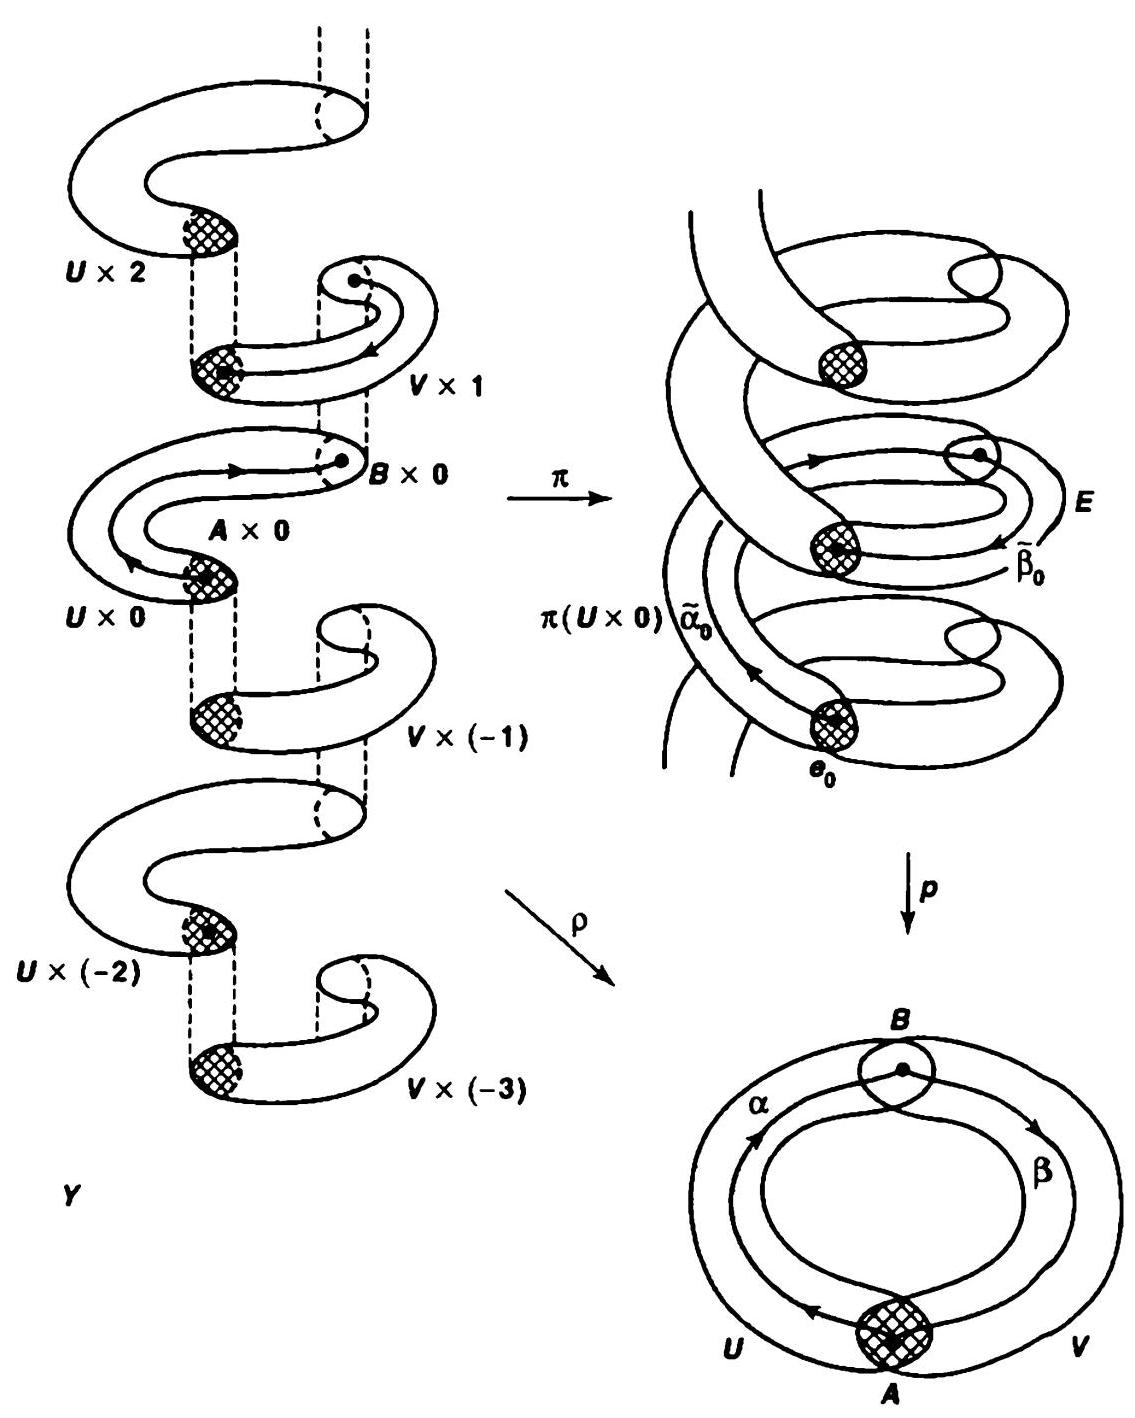
\includegraphics[width=1.0\textwidth]{images/63.1.jpg}
\end{center}
\hspace*{3em} 

Figure 63.1

Step 3. We show that \([  f]\) generates an infinite cyclic subgroup of \({\pi }_{1}( {X,a})\) . It suffices to show that if \(m\) is a positive integer, then \({[  f]  }^{m}\) is not the identity element. But this is easy. For the product

\[
\widetilde{h} = {\bar{f}}_{0} * ( {{\bar{f}}_{1} * ( {\cdots  * {\bar{f}}_{m - 1}}) })
\]

is defined and is a lifting of the \(m\) -fold product

\[
h = f * ( {f * ( {\cdots  * f}) }) .
\]

Because \(\bar{h}\) begins at \({e}_{0}\) and ends at \({e}_{m}\) , the class \([  h] = {[  f]  }^{m}\) cannot be trivial.

*Step 4. Now we show that if \({\pi }_{1}( {X,a})\) is infinite cyclic, it is generated by \([  f]\) . Consider the lifting correspondence \(\phi  : {\pi }_{1}( {X,a})  \rightarrow  {p}^{-1}( a)\) . We showed in Step 3 that for each positive integer \(m\) , the correspondence \(\phi\) carries \({[  f]  }^{m}\) to the point \({e}_{m}\) of \({p}^{-1}( a)\) . A similar argument shows that it carries \({[  f]  }^{-m}\) to \({e}_{-m}\) . Thus \(\phi\) is surjective. Now by Theorem 54.6, \(\phi\) induces an injective map

\[
\Phi  : {\pi }_{1}( {X,a}) /H \rightarrow  {p}^{-1}( a)
\]

where \(H = {p}_{ * }( {{\pi }_{1}( {E,{e}_{0}}) })\) ; the map \(\Phi\) is surjective because \(\phi\) is surjective. It follows that \(H\) is the trivial group, since the quotient of an infinite cyclic group by any nontrivial subgroup is finite. Then the lifting correspondence \(\phi\) itself is bijective; since it maps the subgroup generated by \([  f]\) onto \({p}^{-1}( a)\) , this subgroup must equal all of \({\pi }_{1}( {X,a})\) .

Step 5. Now we prove (c). The picture in Figure 63.1 may mislead you into thinking that the element \([  g]\) of \({\pi }_{1}( {X,a})\) considered in part (c) is in fact trivial. But that figure is rather special. Figure 63.2 illustrates what can occur when \(A\) is itself the union of two disjoint nonempty open sets. In this case (which will be useful to us shortly) both \([  f]\) and \([  g]\) generate infinite cyclic subgroups of \({\pi }_{1}( {X,a})\) .

\begin{center}
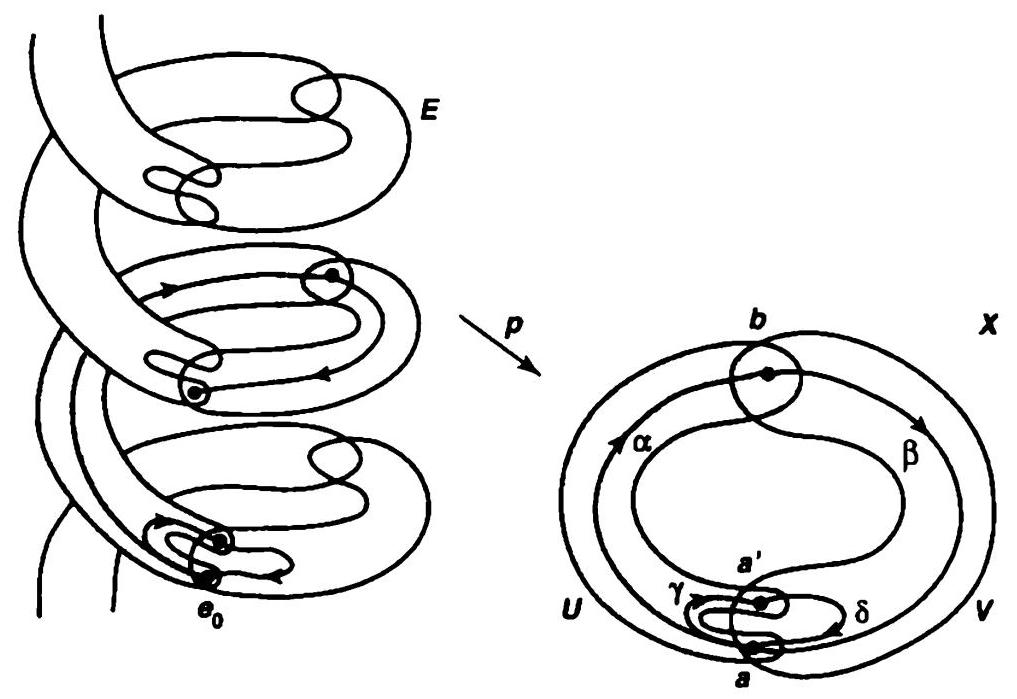
\includegraphics[width=0.9\textwidth]{images/63.2.jpg}
\end{center}
\hspace*{3em} 

Figure 63.2

Given \(g = \gamma  * \delta\) , we define a lifting of \(g\) to \(E\) as follows: Since \(\gamma\) is a path in \(U\) , we can define

\[
\widetilde{\gamma }( s)  = \pi ( {\gamma ( s)  \times  0}) ;
\]

since \(\delta\) is a path in \(V\) , we can define

\[
\widetilde{\delta }( s)  = \pi ( {\delta ( s)  \times  ( {-1}) }) .
\]

Then \(\widetilde{\gamma }\) and \(\widetilde{\delta }\) are liftings of \(\gamma\) and \(\delta\) . The product \(\bar{g} = \widetilde{\gamma } * \widetilde{\delta }\) is defined, since \(\widetilde{\gamma }\) ends at \(\pi ( {{a}^{\prime } \times  0})\) and \(\widetilde{\delta }\) begins at \(\pi ( {{a}^{\prime } \times  ( {-1}) })\) ; and it is a lifting of \(g\) . Note that \(\bar{g}\) is a loop in \(E\) , for it begins and ends at \(\pi ( {a \times  0})  = \pi ( {a \times  ( {-1}) })  = {e}_{0}\) .

It follows that the subgroups generated by \([  f]\) and \([  g]\) have only the identity element in common. For the \(m\) -fold product of \(f\) with itself lifts to a path that begins at \({e}_{0}\) and ends at \({e}_{m}\) , while every product of \(g\) with itself lifts to a path beginning and ending at \({e}_{0}\) . Hence \({[  f]  }^{m} \neq  {[  g]  }^{k}\) for every nonzero \(m\) and \(k\) .
\end{proof}
\begin{theorem}[A nonseparation theorem]
	Let \(D\) be an arc in \({S}^{2}\) . Then \(D\) \index{Arc!does not separate \({S}^{2}\)}does not separate \({S}^{2}\) .
\end{theorem}

\begin{proof}
	We give two proofs of this theorem. The first uses the results of the preceding section, and the second does not.
First proof. Because \(D\) is contractible, the identity map i : \(D \rightarrow  D\) is nulhomo-topic. Hence if \(a\) and \(b\) are any two points of \({S}^{2}\) not in \(D\) , the inclusion \(j : D \rightarrow\)  \({S}^{2} - a - b\) is nulhomotopic. The \index{borsuk lemma@Borsuk lemma}Borsuk lemma then implies that \(a\) and \(b\) lie in the same component of \({S}^{2} - D\) .

Second Proof. Let us write \(D\) as the union of two arcs \({D}_{1}\) and \({D}_{2}\) that intersect in a single point \(d\) . Let \(a\) and \(b\) be points not in \(D\) . We show that if \(a\) and \(b\) can be joined by paths in \({S}^{2} - {D}_{1}\) and in \({S}^{2} - {D}_{2}\) , then they can be joined by a path in \({S}^{2} - D\) . Figure 63.3 illustrates the fact that this assertion is not entirely trivial.

\begin{center}
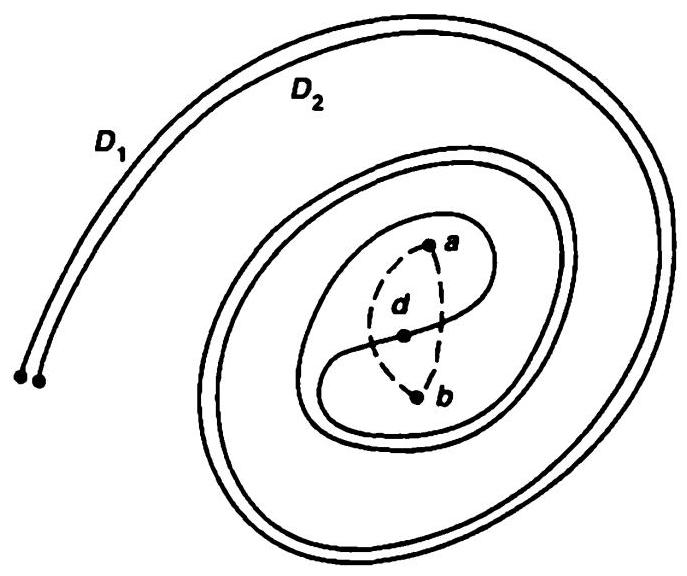
\includegraphics[width=0.6\textwidth]{images/63.3.jpg}
\end{center}
\hspace*{3em} 

Figure 63.3

We suppose that \(a\) and \(b\) cannot be joined by a path in \({S}^{2} - D\) and derive a contradiction. We apply Theorem 63.1. Let \(X\) be the space \({S}^{2} - d\) . Let \(U\) and \(V\) be the open sets

\[
U = {S}^{2} - {D}_{1}\;\text{ and }\;V = {S}^{2} - {D}_{2}.
\]

Then \(X = U \cup  V\) , and \(U \cap  V = {S}^{2} - D\) . By hypothesis, \(a\) and \(b\) are points of \({S}^{2} - D\) that cannot be joined by a path in \({S}^{2} - D\) . Therefore, \(U \cap  V\) is not path connected. Let \(A\) be the path component of \(U \cap  V\) containing \(a\) ; let \(B\) be the union of the other path components of \(U \cap  V\) . Since \(U \cap  V\) is locally path connected (being open in \({S}^{2}\) ), the path components of \(U \cap  V\) are open; hence \(A\) and \(B\) are open in \(X\) . We are given that \(a\) and \(b\) can be joined by paths in \(U = {S}^{2} - {D}_{1}\) and \(V = {S}^{2} - {D}_{2}\) . We conclude from Theorem 63.1 that \({\pi }_{1}( {X,a})\) is not trivial. But \(X = {S}^{2} - d\) , so its fundamental group is trivial.

Now we prove the theorem Given the arc \(D\) and the points \(a\) and \(b\) of \({S}^{2} - D\) , we suppose that \(a\) and \(b\) cannot be joined by a path in \({S}^{2} - D\) and derive a contradiction. Choose a homeomorphism \(h : [  {0,1}] \rightarrow  D\) ; let \({D}_{1} = h( [  {0,1/2}]  )\) and \({D}_{2} = h( [  {1/2,1}]  )\) . The result of the preceding paragraph shows that since \(a\) and \(b\) cannot be joined by a path in \({S}^{2} - D\) , they cannot be joined by paths in both \({S}^{2} - {D}_{1}\) and \({S}^{2} - {D}_{2}\) . To be definite, suppose that \(a\) and \(b\) cannot be joined by a path in \({S}^{2} - {D}_{1}\) .

Now repeat the argument, breaking \({D}_{1}\) up into two arcs \({E}_{1} = h( [  {0,1/4}]  )\) and \({E}_{2} = h( [  {1/4,1/2}]  )\) . We conclude, as before, that \(a\) and \(b\) cannot be joined by paths in both \({S}^{2} - {E}_{1}\) and \({S}^{2} - {E}_{2}\)

Contune similarly. In this way we define a sequence

\[
I \supset  {I}_{1} \supset  {I}_{2} \supset  \cdots
\]

of closed intervals such that \({I}_{n}\) has length \({( 1/2) }^{n}\) and such that for each \(n\) , the points \(a\) and \(b\) cannot be joined by a path in \({S}^{2} - h( {I}_{n})\) . Compactness of the unit interval guarantees there is a point \(x\) in \(\bigcap {I}_{n}\) ; since the lengths of the intervals converge to zero, there is only one such point.

Consider the space \({S}^{2} - h( x)\) . Since this space is homeomorphic to \({\mathbb{R}}^{2}\) , the points \(a\) and \(b\) can be joined by a path \(\alpha\) in \({S}^{2} - h( x)\) . Because \(\alpha ( I)\) is compact, it is closed, so some \(\epsilon\) -neighborhood of \(h( x)\) is disjoint from \(\alpha ( I)\) . Then because \(h\) is continuous, there is some \(m\) such that \(h( {I}_{m})\) lies in this \(\epsilon\) -neighborhood. It follows that \(\alpha\) is a path in \({S}^{2} - h( {I}_{m})\) joining \(a\) and \(b\) , contrary to hypothesis.

Both proofs of this theorem are interesting. As we noted in  \S 62, the first generalizes to show that no compact contractible subspace of \({S}^{2}\) separates \({S}^{2}\) . The second generalizes in another direction. Let us examine this second proof, and ask ourselves what properties of the sets \({D}_{1}\) and \({D}_{2}\) made it work? One readily sees that all that was needed was the fact that \({D}_{1}\) and \({D}_{2}\) were closed subsets of \({S}^{2}\) and that \({S}^{2} - ( {{D}_{1} \cap  {D}_{2}})\) was simply connected. Hence we have the following result, which we shall use later:
\end{proof}
\begin{theorem}[A \index{General nonseparation theorem}]
	Let \({D}_{1}\) and \({D}_{2}\) be closed subsets of \({S}^{2}\) such that \({S}^{2} - {D}_{1} \cap  {D}_{2}\) is simply connected. If neither \({D}_{1}\) nor \({D}_{2}\) separates \({S}^{2}\) , then \({D}_{1} \cup  {D}_{2}\) does not separate \({S}^{2}\) .
\end{theorem}

Now we prove the Jordan curve theorem.

\begin{theorem}[The Jordan curve theorem]
	Let \(C\) be a simple closed curve in \({S}^{2}\) . Then \(C\) separates \({S}^{2}\) into precisely two components \({W}_{1}\) and \({W}_{2}\) . Each of the sets \({W}_{1}\) and \({W}_{2}\) has \(C\) as its boundary; that is, \(C = {\bar{W}}_{i} - {W}_{i}\) for \(\mathrm{i} = 1,2\) .
\end{theorem}

\begin{proof}
	Step 1. We first prove that \({S}^{2} - C\) has precisely two components. Write \(C\) as the union of two arcs \({C}_{1}\) and \({C}_{2}\) that intersect in a two-point set \(\{ p,q\}\) . Let \(X\) be the space \({S}^{2} - p - q\) , and let \(U\) and \(V\) be the open sets
\[
U = {S}^{2} - {C}_{1}\;\text{ and }\;V = {S}^{2} - {C}_{2}.
\]

Then \(X = U \cup  V\) , and \(U \cap  V = {S}^{2} - C\) . The space \(U \cap  V\) has at least two components, by the Jordan separation theorem.

We suppose that \(U \cap  V\) has more than two components and derive a contradiction. Let \({A}_{1}\) and \({A}_{2}\) be two of the components of \(U \cap  V\) , and let \(B\) be the union of the others. Because \({S}^{2} - C\) is locally connected, each of these sets is open. Let \(a \in  {A}_{1}\) and \({a}^{\prime } \in  {A}_{2}\) and \(b \in  B\) . Because the arcs \({C}_{1}\) and \({C}_{2}\) do not separate \({S}^{2}\) , there are paths \(\alpha\) and \(\gamma\) in \(U\) from \(a\) to \(b\) and from \(a\) to \({a}^{\prime }\) , respectively, and there are paths \(\beta\) and \(\delta\) in \(V\) from \(b\) to \(a\) and from \({a}^{\prime }\) to \(a\) , respectively. Consider the loops \(f = \alpha  * \beta\) and \(g = \gamma  * \delta\) . Writing \(U \cap  V\) as the union of the open sets \({A}_{1} \cup  {A}_{2}\) and \(B\) , we see that Theorem 63.1 implies that \([  f]\) is a nontrivial element of \({\pi }_{1}( {X,a})\) . Writing \(U \cap  V\) as the union of the disjoint open sets \({A}_{1}\) and \({A}_{2} \cup  B\) , we see that \([  g]\) is also a nontrivial element of \({\pi }_{1}( {X,a})\) . Since \({\pi }_{1}( {X,a})\) is infinite cyclic, we must have \({[  f]  }^{m} = {[  g]  }^{k}\) for some nonzero integers \(m\) and \(k\) . This result contradicts (c) of Theorem 63.1 .

Step 2. Now we show that \(C\) is the common boundary of \({W}_{1}\) and \({W}_{2}\)

Because \({S}^{2}\) is locally connected, each of the components \({W}_{1}\) and \({W}_{2}\) of \({S}^{2} - C\) is open in \({S}^{2}\) . In particular, neither contains a limit point of the other, so that both the sets \({\bar{W}}_{1} - {W}_{1}\) and \({\bar{W}}_{2} - {W}_{2}\) must be contained in \(C\) .

To prove the reverse inclusion, we show that if \(x\) is a point of \(C\) , every neighborhood \(U\) of \(x\) intersects the closed set \({\bar{W}}_{1} - {W}_{1}\) . It follows that \(x\) is in the set \({\bar{W}}_{1} - {W}_{1}\) .

So let \(U\) be a neighborhood of \(x\) . Because \(C\) is homeomorphic to the circle \({S}^{1}\) , we can break \(C\) up into two arcs \({C}_{1}\) and \({C}_{2}\) that intersect in only their end points, such that \({C}_{1}\) is small enough that it lies inside \(U\) . See Figure 63.4.

\begin{center}
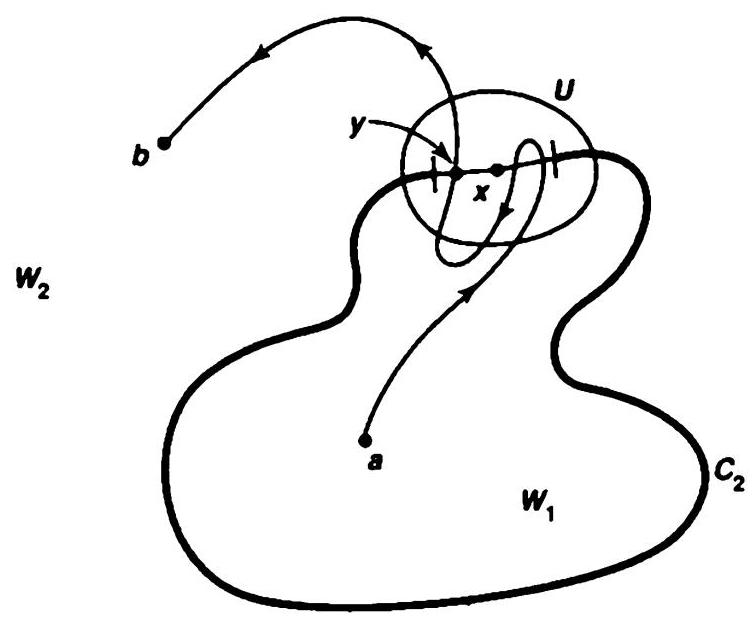
\includegraphics[width=0.7\textwidth]{images/63.4.jpg}
\end{center}
\hspace*{3em} 

Figure 63.4

Let \(a\) and \(b\) be points of \({W}_{1}\) and \({W}_{2}\) , respectively. Because \({C}_{2}\) does not separate \({S}^{2}\) , we can find a path \(\alpha\) in \({S}^{2} - {C}_{2}\) joining \(a\) and \(b\) . The set \(\alpha ( I)\) must contain a point \(y\) of the set \({\bar{W}}_{1} - {W}_{1}\) , because otherwise \(\alpha ( I)\) would be a connected set lying in the union of the disjoint open sets \({W}_{1}\) and \({S}^{2} - {\bar{W}}_{1}\) , and intersecting each of them. The point \(y\) belongs to the closed curve \(C\) , since \(( {{\bar{W}}_{1} - {W}_{1}})  \subset  C\) . Because the path \(\alpha\) does not intersect the arc \({C}_{2}\) , the point \(y\) must therefore lie in the arc \({C}_{1}\) , which in turn lies in the open set \(U\) . Thus, \(U\) intersects \({\bar{W}}_{1} - {W}_{1}\) in the point \(y\) , as desired.

Just as with the earlier theorems, we now ask ourselves what made the proof of this theorem work. Examining Step 1 of the proof, we see that all we used were the facts that \({C}_{1}\) and \({C}_{2}\) were closed connected sets, that \({C}_{1} \cap  {C}_{2}\) consisted of two points, and that neither \({C}_{1}\) nor \({C}_{2}\) separated \({S}^{2}\) . The first two facts implied that \({C}_{1} \cup  {C}_{2}\) separated \({S}^{2}\) into at least two components; the third implied that there were only two components. Hence one has, with no further effort, the following result:
\end{proof}
\begin{theorem}
	Let \({C}_{1}\) and \({C}_{2}\) be closed connected subsets of \({S}^{2}\) whose intersection consists of two points. If neither \({C}_{1}\) nor \({C}_{2}\) separates \({S}^{2}\) , then \({C}_{1} \cup  {C}_{2}\) separates \({S}^{2}\) into precisely two components.
\end{theorem}

Example 1. The second half of the Jordan curve theorem, to the effect that \(C\) is the common boundary of \({W}_{1}\) and \({W}_{2}\) , may seem so obvious as hardly to require comment. But it depends crucially on the fact that \(C\) is homeomorphic to \({S}^{1}\) .

For instance, consider the space indicated in Figure 63 5. It is the union of two arcs whose intersection consists of two points, so it separates \({S}^{2}\) into two components \({W}_{1}\) and \({W}_{2}\) just as the circle does, by Theorem 63.5. But \(C\) does not equal the common boundary of \({W}_{1}\) and \({W}_{2}\) in this case.

\begin{center}
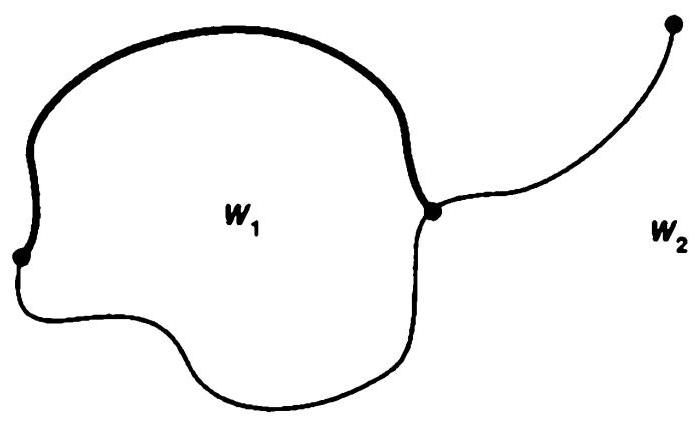
\includegraphics[width=0.6\textwidth]{images/63.5.jpg}
\end{center}
\hspace*{3em} 

Figure 63.5

There is a fourth theorem that is often considered along with these three separation theorems. It is called the \index{schoenflies theorem@Schoenflies theorem}, and it states that if \(C\) is a simple closed curve in \({S}^{2}\) and \(U\) and \(V\) are the components of \({S}^{2} - C\) , then \(\bar{U}\) and \(\bar{V}\) are each homeomorphic to the closed unit ball \({B}^{2}\) . A proof may be found in 		\cite{HallSpencer1955}.

The separation theorems can be generalized to higher dimensions as follows: (1) Any subspace \(C\) of \({S}^{n}\) homeomorphic to \({S}^{n - 1}\) separates \({S}^{n}\) .

(2) No subspace \(A\) of \({S}^{n}\) homeomorphic to \([  {0,1}]\) or to some ball \({B}^{m}\) separates \({S}^{n}\) .

(3) Any subspace \(C\) of \({S}^{n}\) homeomorphic to \({S}^{n - 1}\) separates \({S}^{n}\) into two components, of which \(C\) is the common boundary.

These theorems can be proved quite readily once one has studied singular homology groups in algebraic topology. (See 		\cite{Munkres1993}, p. 202.) The Brouwer theorem on invariance of domain for \({\mathbb{R}}^{n}\) follows as a corollary.

The \index{schoenflies theorem@Schoenflies theorem}Schoenflies theorem, however, does not generalize to higher dimensions without some restrictions on the way the space \(C\) is imbedded in \({S}^{n}\) . This is shown by the famous example of the ``\index{alexander horned sphere@Alexander horned sphere},'' a homeomorphic image of \({S}^{2}\) in \({S}^{3}\) , one of whose complementary domains is not simply connected! (See 		\cite{HockingYoung1961}, p. 176.)

The separation theorems can be generalized even further than this. The definitive theorem along these lines is the famous Alexander-Pontryagin duality theorem, a rather deep theorem of algebraic topology, which we shall not attempt to state here. (See 		\cite{Munkres1993}.) It implies that if the closed subspace \(C\) separates \({S}^{n}\) into \(k\) components, so does any subspace of \({S}^{n}\) that is homeomorphic to \(C\) (or even homotopy equivalent to \(C\) ). The separation theorems (1)-(3) are immediate corollaries.

\section*{Exercises}
\begin{enumerate}[itemsep=0.4em, parsep=0pt, topsep=0pt, partopsep=0pt, leftmargin=*, label=\arabic*., ref=\arabic*]
\item Let \({C}_{1}\) and \({C}_{2}\) be disjoint simple closed curves in \({S}^{2}\) .
  \begin{enumerate}[itemsep=0.2em, parsep=0pt, topsep=0pt, partopsep=0pt, leftmargin=*, label=(\alph*), align=left]
  \item Show that \({S}^{2} - {C}_{1} - {C}_{2}\) has precisely three components. [Hint: If \({W}_{1}\) is the component of \({S}^{2} - {C}_{1}\) disjoint from \({C}_{2}\) , and if \({W}_{2}\) is the component of \({S}^{2} - {C}_{2}\) disjoint from \({C}_{1}\) , show that \({\bar{W}}_{1} \cup  {\bar{W}}_{2}\) does not separate \({S}^{2}\) .]
  \item Show that these three components have boundaries \({C}_{1}\) and \({C}_{2}\) and \({C}_{1} \cup  {C}_{2}\) , respectively.
  \end{enumerate}
\item Let \(D\) be a closed connected subspace of \({S}^{2}\) that separates \({S}^{2}\) into \(n\) components.
  \begin{enumerate}[itemsep=0.2em, parsep=0pt, topsep=0pt, partopsep=0pt, leftmargin=*, label=(\alph*), align=left]
  \item If \(A\) is an arc in \({S}^{2}\) whose intersection with \(D\) consists of one of its end points, show that \(D \cup  A\) separates \({S}^{2}\) into \(n\) components.
  \item If \(A\) is an arc in \({S}^{2}\) whose intersection with \(D\) consists of its end points, show that \(D \cup  A\) separates \({S}^{2}\) into \(n + 1\) components.
  \item If \(C\) is a simple closed curve in \({S}^{2}\) that intersects \(D\) in a single point, show \(D \cup  C\) separates \({S}^{2}\) into \(n + 1\) components. *3. (a) Let \(D\) be a subspace of \({S}^{2}\) homeomorphic to the \index{Topologist's sine curve!does not separate \({S}^{2}\)}topologist's sine curve \(\bar{S}\) . (See  \S 24.) Show that \(D\) does not separate \({S}^{2}\) . [Hint: Let \(h : \bar{S} \rightarrow  D\) be the homeomorphism. Given \(0 < c < 1\) , let \({\bar{S}}_{c}\) equal the intersection of \(\bar{S}\) with the set \(\{ ( {x,y})  \mid  x \leq  c\}\) . Show that given \(a,b \in  {S}^{2} - D\) , there is, for some value of \(c\) , a path in \({S}^{2} - h( {\bar{S}}_{c})\) from \(a\) to \(b\) . Conclude that there is a path in \({S}^{2} - D\) from \(a\) to \(b\) .]
  \item Let \(C\) be a subspace of \({S}^{2}\) homeomorphic to the closed topologist's sine curve. Show that \(C\) separates \({S}^{2}\) into precisely two components, of which \(C\) is the common boundary. [Hint: Let \(h\) be the homeomorphism of the closed topologist's sine curve with \(C\) . Let \({C}_{0} = h( {0\times \lbrack  - 1,1\rbrack })\) . Show first, using the argument of Theorem 63.4, that each point of \(C - {C}_{0}\) lies in the boundary of each component of \({S}^{2} - C\) .]
  \end{enumerate}
\end{enumerate}
\section*{§ 64 Imbedding Graphs in the Plane}

A (finite) linear graph \(G\) is a Hausdorff space that is written as the union of finitely many arcs, each pair of which intersect in at most a common end point. The arcs are called the edges of the graph, and the end points of the arcs are called the vertices of the graph.

Linear graphs are used in mathematics to model many real-life phenomena; however, we shall look at them simply as interesting spaces that in some sense are generalizations \index{Winding number!of simple closed curve}of simple closed curves.

Note that any graph is determined completely (up to homeomorphism) by listing its vertices and specifying which pairs of vertices have an edge joining them.

\begin{centeredblock}
\begin{example}
	If \(G\) contains exactly \(n\) vertices, and if for every pair of distinct vertices of \(G\) there is an edge of \(G\) joining them, then \(G\) is called the \index{Complete graph} on \(n\) vertices and is denoted \({G}_{n}\) . Several such graphs are pictured in Figure 64.1. Note that the first three of these graphs are pictured as subspaces of \({\mathbb{R}}^{2}\) , but the fourth is pictured instead as a subspace of \({\mathbb{R}}^{3}\) . A little experimentation will convince you that this graph cannot in fact be imbedded in \({\mathbb{R}}^{2}\) . We shall prove this result shortly.

\begin{center}
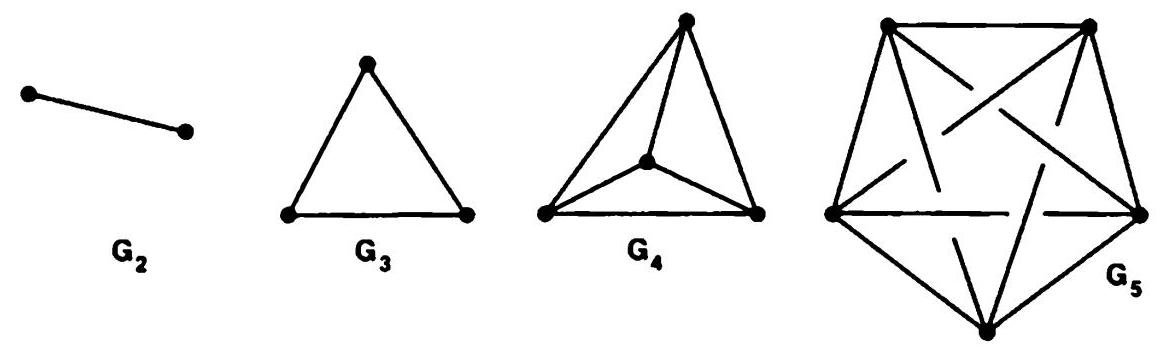
\includegraphics[width=1.0\textwidth]{images/64.1.jpg}
\end{center}
\hspace*{3em}

Figure 64.1
\end{example}
\end{centeredblock}

\begin{centeredblock}
\begin{example}
	Another interesting graph arises in considering the classical puzzle: ``Given three houses, \({h}_{1},{h}_{2}\) , and \({h}_{3}\) , and three utilities, \(g\) (for gas), \(w\) (for water), and \(e\) (for electricity), can you connect each utility to each house without letting any of the connecting lines cross?'' Formulated mathematically, this is just the question whether the graph pictured in Figure 64.2, which is called the utilities graph. can be imbedded in \({\mathbb{R}}^{2}\) . Again, a little experimentation will convince you that it cannot, a fact that we shall prove shortly
\end{example}
\end{centeredblock}

\begin{definition}
	A theta space \(X\) is a Hausdorff space that is written as the union of three arcs \(A,B\) , and \(C\) , each pair of which intersect precisely in their end points. (The space \(X\) is of course homeomorphic to the Greek letter theta.)
\end{definition}

\begin{center}
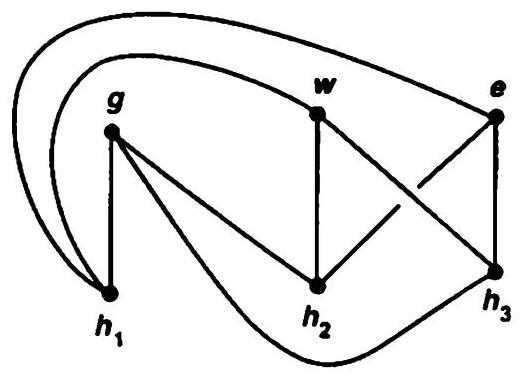
\includegraphics[width=0.4\textwidth]{images/64.2.jpg}
\end{center}
\hspace*{3em} 

Figure 64.2

Note that as it stands, a theta space \(X\) is not a linear graph, for the arcs in question intersect in more than a common end point. One can write it as a graph, however, by breaking each of the arcs \(A,B\) , and \(C\) up into two arcs with an end point in common.

\begin{lemma}
	Let \(X\) be a theta space that is a subspace of \({S}^{2}\) ; let \(A,B\) , and \(C\) be the arcs whose union is \(X\) . Then \(X\) separates \({S}^{2}\) into three components, whose boundaries are \(A \cup  B,B \cup  C\) , and \(A \cup  C\) , respectively. The component having \(A \cup  B\) as its boundary equals one of the components of \({S}^{2} - A \cup  B\) .
\end{lemma}

\begin{proof}
	Let \(a\) and \(b\) be the end points of the arcs \(A,B\) , and \(C\) . Consider the simple closed curve \(A \cup  B\) ; it separates \({S}^{2}\) into two components \(U\) and \({U}^{\prime }\) , each of which is open in \({S}^{2}\) and has boundary \(A \cup  B\) . See Figure 64.3.
\begin{center}
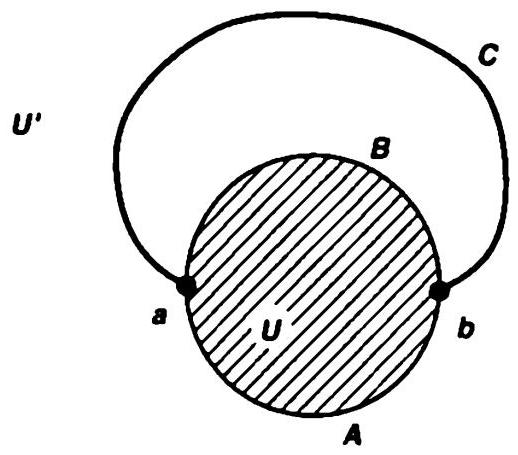
\includegraphics[width=0.4\textwidth]{images/64.3.jpg}
\end{center}
\hspace*{3em} 

Figure 64.3

The space \(C - a - b\) is connected, so it is contained in one of these components, say in \({U}^{\prime }\) . Then consider the two spaces \(\widetilde{U} = U \cup  A \cup  B\) and \(C\) ; each is connected. Neither separates \({S}^{2}\) , for \(C\) is an arc, and the complement of \(\widetilde{U}\) is the connected set \({U}^{\prime }\) . Since the intersection of these two sets consists of the two points \(a\) and \(b\) , their union separates \({S}^{2}\) into two components \(V\) and \(W\) , by Theorem 63.5. It follows that \({S}^{2} -\)  \(( {A \cup  B \cup  C})\) is the union of the three disjoint connected sets \(U,V\) , and \(W\) ; because they are open in \({S}^{2}\) , they are the components of \({S}^{2} - ( {A \cup  B \cup  C})\) . The component \(U\) has \(A \cup  B\) as its boundary. Symmetry implies that the other two have \(B \cup  C\) and

\(A \cup  C\) as their boundaries.
\end{proof}
\begin{theorem}
	Let \(X\) be the utilities graph. Then \(X\) \index{Utilities graph!nonembeddability}cannot be imbedded in the plane.
\end{theorem}

\begin{proof}
	If \(X\) can be imbedded in the plane, then it can be imbedded in \({S}^{2}\) . So suppose \(X\) is a subspace of \({S}^{2}\) . We derive a contradiction.
We use the notation of Example 2, where \(g,w,e,{h}_{1},{h}_{2}\) , and \({h}_{3}\) are the vertices of \(X\) . Let \(A,B\) , and \(C\) be the following arcs contained in \(X\) :

\[
\begin{aligned}  & A = g{h}_{1}w, \\  & B = g{h}_{2}w \\  & C = g{h}_{3}w. \end{aligned}
\]

Each pair of these arcs intersect in their end points \(g\) and \(w\) alone; hence \(Y = A \cup  B \cup  C\) is a \index{Theta space!separates \({S}^{2}\)}\index{Separation theorem: closed topologist's sine curve in \({S}^{2}\)!theta space in \({S}^{2}\)}theta space. The space \(Y\) separates \({S}^{2}\) into three components \(U,V\) , and \(W\) , whose boundaries are \(A \cup  B,B \cup  C\) , and \(A \cup  C\) , respectively. See Figure 64.4.

Now the vertex \(e\) of \(X\) lies in one of these three components, so that the arcs \(e{h}_{1}\) and \(e{h}_{2}\) and \(e{h}_{3}\) of \(X\) lie in the closure of that component. That component cannot be \(U\) , for \(\widetilde{U}\) is contained in \(U \cup  A \cup  B\) , a set that does not contain the point \({h}_{3}\) . Similarly, the component containing \(e\) cannot be \(V\) or \(W\) , because \(\widetilde{V}\) does not contain \({h}_{1}\) , and \(\bar{W}\) does not contain \({h}_{2}\) . Thus, we have reached a contradiction.

\begin{center}
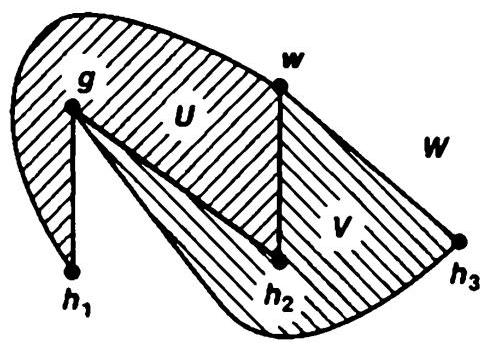
\includegraphics[width=0.4\textwidth]{images/64.4.jpg}
\end{center}
\hspace*{3em} 

Figure 64.4
\end{proof}
\begin{lemma}
	Let \(X\) be a subspace of \({S}^{2}\) that is a \index{complete graph@Complete graph}complete graph on four vertices \({a}_{1}\) , \({a}_{2},{a}_{3}\) , and \({a}_{4}\) . Then \(X\) separates \({S}^{2}\) into four components. The boundaries of these components are the sets \({X}_{1},{X}_{2},{X}_{3}\) , and \({X}_{4}\) , where \({X}_{i}\) is the union of those edges of \(X\) that do not have \({a}_{i}\) as a vertex.
\end{lemma}

\begin{proof}
	Let \(Y\) be the union of all the arcs of \(X\) different from the arc \({a}_{2}{a}_{4}\) . Then we can write \(Y\) as a theta space by setting
\[
\begin{aligned}  & A = {a}_{1}{a}_{2}{a}_{3}, \\  & B = {a}_{1}{a}_{3}, \\  & C = {a}_{1}{a}_{4}{a}_{3}. \end{aligned}
\]

See Figure 64.5. The arcs \(A,B\) , and \(C\) intersect in their end points \({a}_{1}\) and \({a}_{3}\) alone, and their union is \(Y\) .

\begin{center}

\includegraphics[width=0.5\textwidth]{64.5.jpg}
\end{center}
\hspace*{3em} 

Figure 64.5

The space \(Y\) separates \({S}^{2}\) into three components \(U,V\) , and \(W\) , whose boundaries are \(A \cup  B,B \cup  C\) , and \(A \cup  C\) , respectively. The space \({a}_{2}{a}_{4} - {a}_{2} - {a}_{4}\) , being connected, must lie in one of them. It cannot lie in \(U\) , because \(A \cup  B\) does not contain \({a}_{4}\) . And it cannot lie in \(V\) because \(B \cup  C\) does not contain \({a}_{2}\) . Hence it must lie in \(W\) .

Now \(\bar{U} \cup  \bar{V}\) is connected because \(\bar{U}\) and \(\bar{V}\) are connected and have nonempty intersection \(B\) . Furthermore, the set \(\bar{U} \cup  \bar{V}\) does not separate \({S}^{2}\) , because its complement is \(W\) . Similarly, the arc \({a}_{2}{a}_{4}\) is connected and does not separate \({S}^{2}\) . And the sets \({a}_{2}{a}_{4}\) and \(\bar{U} \cup  \bar{V}\) intersect in the points \({a}_{2}\) and \({a}_{4}\) alone. It follows from Theorem 63.5 that \({a}_{2}{a}_{4} \cup  \bar{U} \cup  \bar{V}\) separates \({S}^{2}\) into two components \({W}_{1}\) and \({W}_{2}\) . Then \({S}^{2} - Y\) is the union of the four disjoint connected sets \(U,V,{W}_{1}\) , and \({W}_{2}\) . Since these sets are open, they are the components of \({S}^{2} - Y\) .

Now one of these components, namely \(U\) , has the graph \(A \cup  B = {X}_{4}\) as its boundary. Symmetry implies that the other three have \({X}_{1},{X}_{2}\) , and \({X}_{3}\) as their respective boundaries.
\end{proof}
\begin{theorem}
	The complete graph on five vertices cannot be imbedded in the plane.
\end{theorem}

\begin{proof}
	Suppose that \(G\) is a subspace of \({S}^{2}\) that is a complete graph on the five vertices \({a}_{1},{a}_{2},{a}_{3},{a}_{4}\) , and \({a}_{5}\) . Let \(X\) be the union of those edges of \(G\) that do not have \({a}_{5}\) as a vertex; then \(X\) is a complete graph on four vertices. The space \(X\) separates \({S}^{2}\) into four components, whose respective boundaries are the graphs \({X}_{1},\ldots ,{X}_{4}\) , where \({X}_{i}\) consists of those edges of \(X\) that do not have \({a}_{i}\) as a vertex. Now the point \({a}_{5}\) must lie in one of these four components. It follows that the connected space
\[
{a}_{1}{a}_{5} \cup  {a}_{2}{a}_{5} \cup  {a}_{3}{a}_{5} \cup  {a}_{4}{a}_{5},
\]

which is the union of those edges of \(G\) that have \({a}_{5}\) as a vertex, must lie in the closure of this component. Then all the vertices \({a}_{1},\ldots ,{a}_{4}\) lie in the boundary of this component. But this is impossible, for none of the graphs \({X}_{i}\) contains all four vertices \({a}_{1},\ldots ,{a}_{4}\) . Thus we reach a contradiction.

It follows from these theorems that if a graph \(G\) contains a subgraph that is a utilities graph or a complete graph on five vertices, then \(G\) cannot be imbedded in the plane. It is a remarkable theorem, due to Kuratowski, that the converse is also true! The proof is not easy.
\end{proof}
\section*{Exercise}

1. Let \(X\) be a space that is written as the union of finitely many arcs \({A}_{1},\ldots ,{A}_{n}\) , each pair of which intersect in at most a common end point.

(a) Show that \(X\) is Hausdorff if and only if each arc \({A}_{i}\) is closed in \(X\) .

(b) Give an example to show that \(X\) need not be Hausdorff. [Hint: See Exercise 5 of  \S 36.]

\section*{§ 65 The Winding Number of a Simple Closed Curve}

If \(h : {S}^{1} \rightarrow  {\mathbb{R}}^{2} - 0\) is a continuous map, then the induced homomorphism \({h}_{ * }\) carries a generator of the fundamental group of \({S}^{1}\) to some integral power of a generator of the fundamental group of \({\mathbb{R}}^{2} - \mathbf{0}\) . This integral power \(n\) is called the \index{Simple closed curve!winding number}winding number of \(h\) with respect to 0. It measures how many times \(h\) ``wraps \({S}^{1}\) around the origin;'' its sign depends of course on the choice of generators. See Figure 65.1. We will introduce it more formally in the next section.

\begin{center}
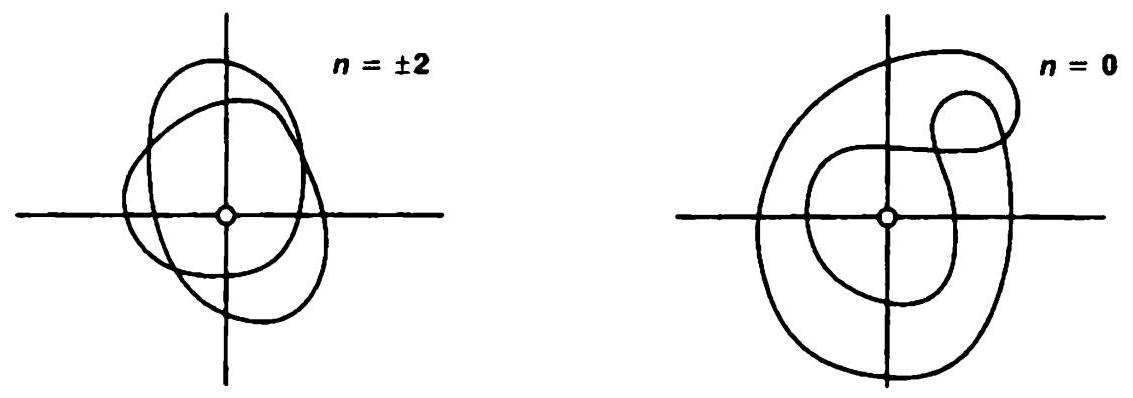
\includegraphics[width=1.0\textwidth]{images/65.1.jpg}
\end{center}
\hspace*{3em} 

Figure 65.1

For the present, we merely ask the question: What can one say about the winding number of \(h\) if \(h\) is injective, that is, if \(h\) is a homeomorphism of \({S}^{1}\) with a simple closed curve \(C\) in \({\mathbb{R}}^{2} - 0\) ? The illustrations in Figure 65.2 suggest the obvious conjecture: If 0 belongs to the unbounded component of \({\mathbb{R}}^{2} - C\) , then \(n = 0\) , while if 0 belongs to the bounded component, then \(n =  \pm  1\) .

\begin{center}
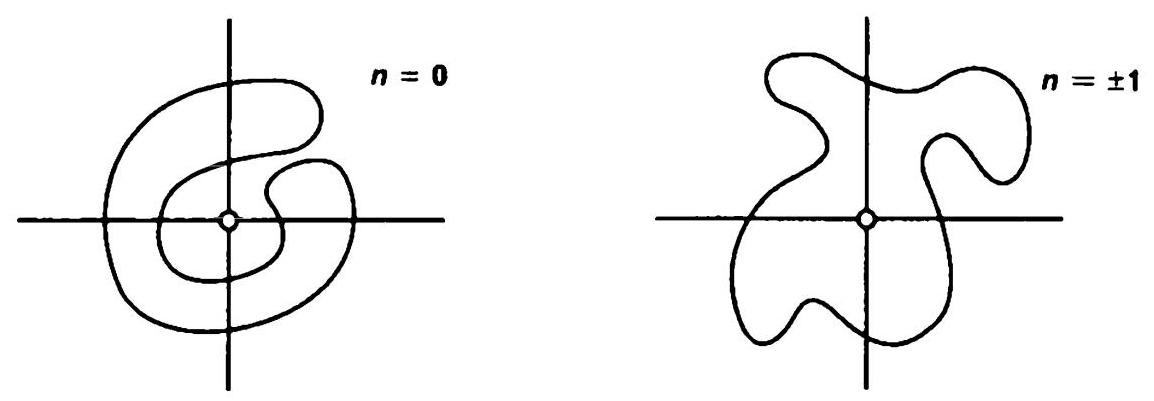
\includegraphics[width=1.0\textwidth]{images/65.2.jpg}
\end{center}
\hspace*{3em} 

Figure 65.2

The first conjecture is easy to prove, for Lemma 61.2 tells us that \(h\) is nulhomotopic if 0 belongs to the unbounded component of \({\mathbb{R}}^{2} - C\) . On the other hand, the second conjecture is surprisingly difficult; it is in fact a rather deep result. We prove it in this section.

As usual, we shall replace \({\mathbb{R}}^{2} \cup  \{ \infty \}\) by \({S}^{2}\) , letting \(p\) be the point corresponding to 0 and \(q\) be the point corresponding to \(\infty\) . Then our conjecture can be reformulated as follows: If \(C\) is a simple closed curve in \({S}^{2}\) , and if \(p\) and \(q\) belong to different components of \({S}^{2} - C\) , then the inclusion mapping \(j : C \rightarrow  {S}^{2} - p - q\) induces an isomorphism of fundamental groups. This is what we shall prove.

First, we prove our result in the case where the simple closed curve \(C\) is contained in a complete graph on four vertices. Then we prove the general case.

\begin{lemma}
	Let \(G\) be a subspace of \({S}^{2}\) that is a complete graph on four vertices \({a}_{1},\ldots ,{a}_{4}\) . Let \(C\) be the subgraph \({a}_{1}{a}_{2}{a}_{3}{a}_{4}{a}_{1}\) , which is a simple closed curve. Let \(p\) and \(q\) be interior points of the edges \({a}_{1}{a}_{3}\) and \({a}_{2}{a}_{4}\) , respectively. Then:

(a) The points \(p\) and \(q\) lie in different components of \({S}^{2} - C\) .

(b) The inclusion \(j : C \rightarrow  {S}^{2} - p - q\) induces an isomorphism of fundamental groups.
\end{lemma}

\begin{proof}
	(a) As in the proof of Lemma 64.3, the theta space \(C \cup  {a}_{1}{a}_{3}\) separates \({S}^{2}\) into three components \(U,V\) , and \(W\) . One of these, say \(W\) , has \(C\) as its boundary; it is the only component whose boundary contains both \({a}_{2}\) and \({a}_{4}\) . Therefore, \({a}_{2}{a}_{4} - {a}_{2} - {a}_{4}\) must lie in \(W\) , so that in partucular, \(q\) belongs to \(W\) . Of course, \(p\) is not in \(W\) because \(p\) belongs to the theta space \(C \cup  {a}_{1}{a}_{3}\) . Now Lemma 64.1 tells us that \(W\) is one of the components of \({S}^{2} - C\) ; therefore, \(p\) and \(q\) belong to different components of \({S}^{2} - C\) .
(b) Let \(X = {S}^{2} - p - q\) . The idea of the proof is the following: We choose a point \(x\) interior to the arc \({a}_{1}{a}_{2}\) , and a point \(y\) interior to the arc \({a}_{3}{a}_{4}\) . And we let \(\alpha\) and \(\beta\) be the broken-line paths

\[
\alpha  = x{a}_{1}{a}_{4}y\;\text{ and }\;\beta  = y{a}_{3}{a}_{2}x.
\]

Then \(\alpha  * \beta\) is a loop lying in the simple closed curve \(C\) . We shall prove that \(\alpha  * \beta\) represents a generator of the fundamental group of \(X\) . It follows that the homomorphism \({j}_{ * } : {\pi }_{1}( {C,x})  \rightarrow  {\pi }_{1}( {X,x})\) is surjective, so that \({j}_{ * }\) must be an isomorphism (since the groups involved are infinite cyclic). See Figure 65.3.

\begin{center}
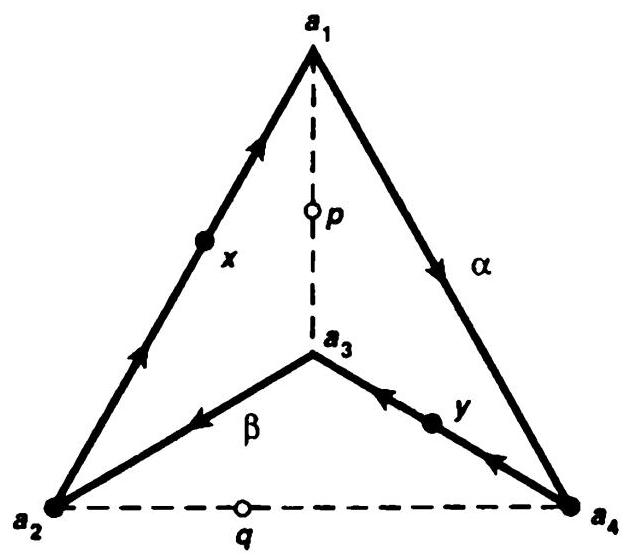
\includegraphics[width=0.5\textwidth]{images/65.3.jpg}
\end{center}
\hspace*{3em} 

Figure 65.3

Let \({D}_{1}\) and \({D}_{2}\) be the arcs

\[
{D}_{1} = p{a}_{3}{a}_{2}q\;\text{ and }\;{D}_{2} = q{a}_{4}{a}_{1}p,
\]

and let \(U = {S}^{2} - {D}_{1}\) and \(V = {S}^{2} - {D}_{2}\) . See Figure 65.4. Then \(X = U \cup  V\) , and \(U \cap  V\) equals \({S}^{2} - D\) , where \(D\) is the simple closed curve \(D = {D}_{1} \cup  {D}_{2}\) . Hence, \(U \cap  V\) has two components, by the Jordan curve theorem. Furthermore, since \(D\) equals the simple closed curve \({a}_{1}{a}_{3}{a}_{2}{a}_{4}{a}_{1}\) , the result of (a) implies that the points \(x\) and \(y\) , which lie interior to the other two edges of the graph \(G\) , lie in different components of \({S}^{2} - D\)

\begin{center}
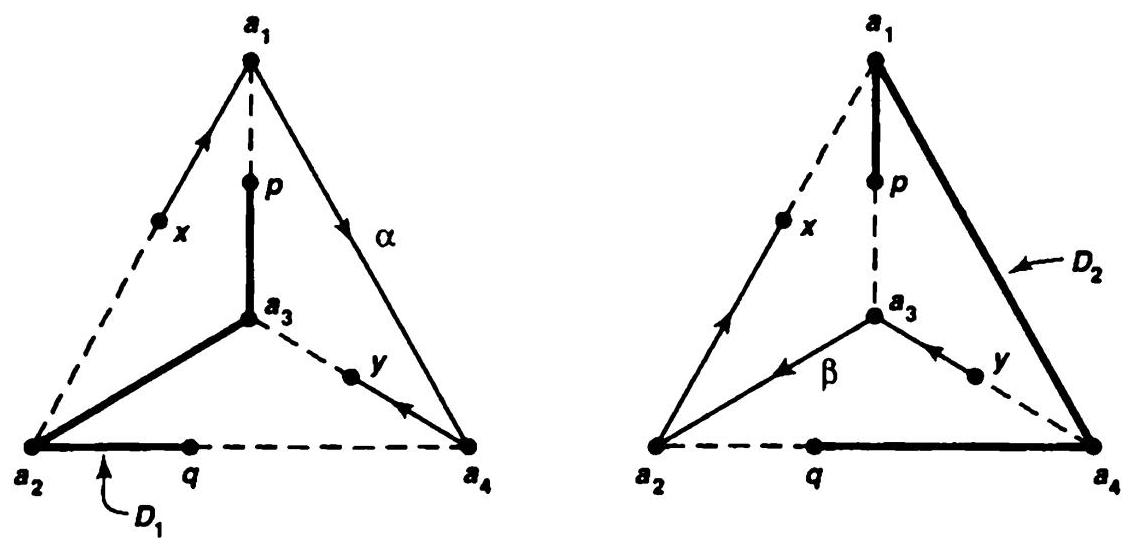
\includegraphics[width=1.0\textwidth]{images/65.4.jpg}
\end{center}
\hspace*{3em} 

Figure 65.4

The hypotheses of Theorem 63.1 are thus satisfied. The path \(\alpha\) is a path in \(U\) from \(x\) to \(y\) , while \(\beta\) is a path in \(V\) from \(y\) to \(x\) . Because the fundamental group of \(X\) is infinite cyclic, the loop \(\alpha  * \beta\) represents a generator of this group.

Now we prove our main theorem.
\end{proof}
\begin{theorem}
	Let \(C\) be a simple closed curve in \({S}^{2}\) ; let \(p\) and \(q\) lie in different components of \({S}^{2} - C\) . Then the inclusion mapping \(j : C \rightarrow  {S}^{2} - p - q\) induces an isomorphism of fundamental groups.
\end{theorem}

\begin{proof}
	The proof involves constructing a complete graph on four vertices that contains \(C\) as a subgraph.
Step 1. Let \(a,b\) , and \(c\) be three distinct points of \({\mathbb{R}}^{2}\) . If \(A\) is an arc with end points points \(a\) and \(b\) , and if \(B\) is an arc with end points \(b\) and \(c\) , then there exists an arc contained in \(A \cup  B\) with end points \(a\) and \(c\) .

Choose paths \(f : I \rightarrow  A\) from \(a\) to \(b\) , and \(g : I \rightarrow  B\) from \(b\) to \(c\) , such that \(f\) and \(g\) are homeomorphisms. Let \({t}_{0}\) be a smallest point of \(I\) such that \(f( {t}_{0})  \in  B\) ; and let \({t}_{1}\) be the point of \(I\) such that \(g( {t}_{1})  = f( {t}_{0})\) . Then the set \(f( [  {0,{t}_{0}}]  )  \cup  g( [  {{t}_{1},1}]  )\) is the required arc. (If \({t}_{0} = 0\) or \({t}_{1} = 1\) , one of these sets consists of a single point.) See Figure 65.5.

\begin{center}
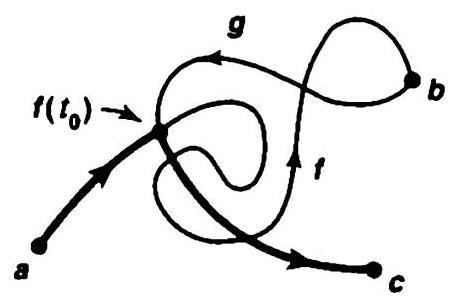
\includegraphics[width=0.4\textwidth]{images/65.5.jpg}
\end{center}
\hspace*{3em} 

Figure 65.5

Step 2. We show that if \(U\) is an open set of \({\mathbb{R}}^{2}\) , any two points of \(U\) that can be connected by a path in \(U\) are the end points of an arc lying in \(U\) .

If \(x,y \in  U\) , set \(x \sim  y\) if \(x = y\) or if there is an arc in \(U\) with end points \(x\) and \(y\) . The result of Step 1 shows that this is an equivalence relation. The equivalence classes are open, for if the \(\epsilon\) -neighborhood of \(x\) lies in \(U\) , it consists of points equivalent to \(x\) . Since \(U\) is connected, there is only one such equivalence class.

Step 3. Let \(C\) be a simple closed curve in \({\mathbb{R}}^{2}\) . We construct a subspace \(G\) of \({\mathbb{R}}^{2}\) that is a complete graph on four vertices \({a}_{1},\ldots ,{a}_{4}\) such that \(C\) equals the subgraph \({a}_{1}{a}_{2}{a}_{3}{a}_{4}{a}_{1}\) .

For convenience, we assume that 0 lies in the bounded component of \({\mathbb{R}}^{2} - C\) . Consider the \(x\) -axis \(\mathbb{R} \times  0\) in \({\mathbb{R}}^{2}\) ; let \({a}_{1}\) be the largest point on the negative \(x\) -axis that lies in \(C\) , and let \({a}_{3}\) be the smallest point on the positive \(x\) -axis that lies in \(C\) . Then the line segment \({a}_{1}{a}_{3}\) lies in the closure of the bounded component of \({\mathbb{R}}^{2} - C\) .

Let us write \(C\) as the union of two arcs \({C}_{1}\) and \({C}_{2}\) with end points \({a}_{1}\) and \({a}_{3}\) . Let \(a\) be a point of the unbounded component of \({\mathbb{R}}^{2} - C\) . Since \({C}_{1}\) and \({C}_{2}\) do not separate \({\mathbb{R}}^{2}\) , we can choose paths \(\alpha  : I \rightarrow  {\mathbb{R}}^{2} - {C}_{1}\) and \(\beta  : I \rightarrow  {\mathbb{R}}^{2} - {C}_{2}\) from \(a\) to 0; in view of Step 2, we may assume that \(\alpha\) and \(\beta\) are injective. Let \({a}_{2} = \alpha ( {t}_{0})\) , where \({t}_{0}\) is the smallest number such that \(\alpha ( {t}_{0})  \in  C\) ; then \({a}_{2}\) is a point interior to \({C}_{2}\) . Similarly, let \({a}_{4} = \beta ( {t}_{1})\) , where \({t}_{1}\) is the smallest number such that \(\beta ( {t}_{1})  \in  C\) ; then \({a}_{4}\) is an interior point of \({C}_{1}\) . Then \(\alpha ( [  {0,{t}_{0}}]  )\) and \(\beta ( [  {0,{t}_{1}}]  )\) are arcs joining \(a\) to \({a}_{2}\) and \({a}_{4}\) , respectively; by Step 2, their union contains an arc with end points \({a}_{2}\) and \({a}_{4}\) ; thus arc intersects \(C\) only in these two points. This arc, along with the line segment \({a}_{1}{a}_{3}\) and the curve \(C\) , forms the desired graph. See Figure 65.6.

\begin{center}
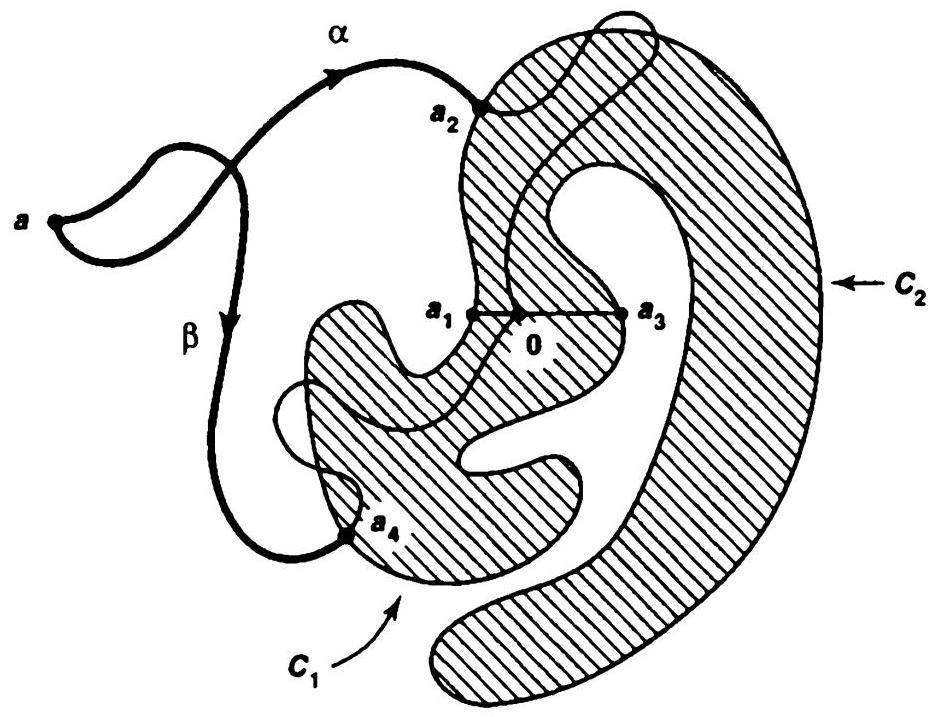
\includegraphics[width=0.8\textwidth]{images/65.6.jpg}
\end{center}
\hspace*{3em} 

Figure 65.6

Step 4. It follows from the result of Step 3 and the preceding lemma that for some pair of points \(p,q\) lying in different components of \({S}^{2} - C\) , the inclusion \(j : C \rightarrow\)  \({S}^{2} - p - q\) induces an isomorphism of fundamental groups. To complete the proof, we need only show that the same holds for any pair \(p,q\) of points lying in different components of \({S}^{2} - C\) . For that purpose, it suffices to prove the following:

Let \(D\) be a simple closed curve in \({\mathbb{R}}^{2}\) ; suppose 0 lies in the bounded component of \({\mathbb{R}}^{2} - D\) . Let \(p\) be another point of this component. If inclusion \(j : D \rightarrow  {\mathbb{R}}^{2} - 0\) induces an isomorphism of fundamental groups, then so does the inclusion \(k : D \rightarrow  {\mathbb{R}}^{2} - p\) .

Let \(f.{\mathbb{R}}^{2} - p \rightarrow  {\mathbb{R}}^{2} - 0\) be the homeomorphism \(f( x)  = x - p\) . It suffices to show that the map

\[
D\overset{k}{ \rightarrow  }{\mathbb{R}}^{2} - p\overset{f}{ \rightarrow  }{\mathbb{R}}^{2} - 0
\]

indices an isomorphism of fundamental groups. Let \(\alpha\) be a path in \({\mathbb{R}}^{2} - D\) from 0 to \(p\) , and let \(F : D \times  I \rightarrow  {\mathbb{R}}^{2} - 0\) be the map \(F( {x,t})  = x - \alpha ( t)\) . Then \(F\) is a homotopy between \(j\) and \(f \circ  k\) ; since \(j\) induces an isomorphism, so does \(f \circ  k\) . (See Corollary 58.5).

This theorem is a special case of a rather deep theorem of algebraic topology, concerning the ``linking number'' of two disjoint subspaces of \({S}^{m + n + 1}\) , one homeomorphic to an \(m\) -sphere and the other homeomorphic to an \(n\) -sphere; it is related to the Alexander duality theorem. (See 		\cite{Munkres1993}, p. 433.) The special case of our theorem is that of a 0-sphere (i.e., a two-point space) and a 1-sphere (i.e., a simple closed curve) in \({S}^{2}\) .
\end{proof}
\section*{§ 66 The Cauchy Integral Formula}

One of the central theorems in the study of functions of a complex variable is the one concerning the Cauchy integral formula for analytic functions. For the classical version of this theorem, one needs to assume not only the Jordan curve theorem, but also the winding-number theorem of the last section. There is, however, a reformulation of the Cauchy integral theorem that avoids using these results; this version of the theorem, although it is rather less natural, is the one now commonly found in texts on the subject.

Since we have the Jordan curve theorem at our disposal, we shall set ourselves the task of deriving the Cauchy integral formula in its classical version from the reformulated version.

We begin by introducing the notion of ``winding number'' more formally.

\begin{definition}
	Let \(f\) be a loop in \({\mathbb{R}}^{2}\) , and let \(a\) be a point not in the image of \(f\) . Set

\[
g( s)  = [  {f( s)  - a}]  /\parallel f( s)  - a\parallel
\]

then \(g\) is a loop in \({S}^{1}\) . Let \(p : \mathbb{R} \rightarrow  {S}^{1}\) be the standard covering map, and let \(\widetilde{g}\) be a lifting of \(g\) to \({S}^{1}\) . Because \(g\) is a loop, the difference \(\widetilde{g}( 1)  - \widetilde{g}( 0)\) is an integer. This integer is called the winding number of \(f\) with respect to \(a\) , and is denoted \(\index{n@\(n( {f,a})\)} n( {f,a})\) .
\end{definition}

Note that \(n( {f,a})\) is independent of the choice of the lifting of \(g\) . For if \(\widetilde{g}\) is one lifting of \(g\) , then uniqueness of liftings implies that any other lifting of \(g\) has the form \(\widetilde{g}( s)  + m\) for some integer \(m\) .

\begin{definition}
	Let \(F : I \times  I \rightarrow  X\) be a continuous map such that \(F( {0,t})  = F( {1,t})\) for all \(t\) . Then for each \(t\) , the map \({f}_{t}( s)  = F( {s,t})\) is a loop in \(X\) . The map \(F\) is called a free homotopy between the loops \({f}_{0}\) and \({f}_{1}\) . It is a homotopy of loops in which the base point of the loop is allowed to move during the homotopy.
\end{definition}

\begin{lemma}
	Let \(f\) be a loop in \({\mathbb{R}}^{2} - a\) .

(a) If \(\bar{f}\) is the reverse of \(f\) , then \(n( {\bar{f},a})  =  - n( {f,a})\) .

(b) If \(f\) is freely homotopic to \({f}^{\prime }\) , through loops lying in \({\mathbb{R}}^{2} - a\) , then \(n( {f,a})  =\)  \(n( {{f}^{\prime },a})\) .

(c) If \(a\) and \(b\) lie in the same component of \({\mathbb{R}}^{2} - f( I)\) , then \(n( {f,a})  = n( {f,b})\) .
\end{lemma}

\begin{proof}
	(a) To compute \(n( {\bar{f},a})\) , one replace \(s\) by \(1 - s\) throughout the definition. This has the effect of changing \(\widetilde{g}( 1)  - \widetilde{g}( 0)\) by a sign
(b) Let \(F\) be a free homotopy between \(f\) and \({f}^{\prime }\) . Define \(G : 1 \times  I \rightarrow  {S}^{1}\) by the equation

\[
G( {s,t})  = [  {F( {s,t})  - a}]  /\parallel F( {s,t})  - a\parallel .
\]

Let \(\bar{G}\) be a lifting of \(G\) to \(\mathbb{R}\) . Then \(\widetilde{G}( {1,t})  - \widetilde{G}( {0,t})\) is an integer for each \(t\) ; being continuous, it is constant.

(c) Let \(\alpha\) be a path in \({\mathbb{R}}^{2} - f( l)\) from \(a\) to \(b\) . Note that by definition, \(n( {f,a})  =\)  \(n( {f - a,0})\) . Since \(f( s)  - \alpha ( t)\) is a free homotopy in \({\mathbb{R}}^{2} - 0\) between \(f - a\) and \(f - b\) , our result follows.
\end{proof}
\begin{definition}
	Let \(f\) be a loop in \(X\) . We call \(f\) a \index{Simple loop} provided \(f( s)  = f( {s}^{\prime })\) only if \(s = {s}^{\prime }\) or if one of the points \(s,{s}^{\prime }\) is 0 and the other is 1 . If \(f\) is a \index{simple loop@Simple loop}simple loop, its image set is a simple closed curve in \(X\) .
\end{definition}

\begin{theorem}
	Let \(f\) be a simple loop in \({\mathbb{R}}^{2}\) . If a lies in the unbounded component of \({\mathbb{R}}^{2} - f( 1)\) , then \(n( {f,a})  = 0\) ; while if a lies in the bounded component, \(n( {f,a})  =  \pm  1\) .
\end{theorem}

\begin{proof}
	Since \(n( {f,a})  = n( {f - a,0})\) , we may restrict ourselves to the case \(a = 0\) . Furthermore, we may assume that the base point of \(f\) lies on the positive \(x\) -axis. For one can gradually rotate \({\mathbb{R}}^{2} - 0\) until the base point of \(f\) is such a point; this modifies \(f\) by a free homotopy, so it does not affect the conclusion of the theorem.
So let \(f\) be a simple loop in \(X = {\mathbb{R}}^{2} - 0\) based at a point \({x}_{0}\) of the positive \(x\) - axis. Let \(C\) be the simple closed curve \(f( I)\) . We show that if0lies in the bounded component of \({\mathbb{R}}^{2} - C\) , then \([  f]\) \index{Simple closed curve!generates \({\pi }_{1}\) of \({\mathbb{R}}^{2} - 0\)}generates \({\pi }_{1}( {X,{x}_{0}})\) , while if 0 lies in the unbounded component, \([  f]\) is trivial.

The map \(f\) induces, \({via}\) the standard quotient map \(p : I \rightarrow  {S}^{1}\) , a homeomorphism \(h : {S}^{1} \rightarrow  C\) . The element \([  p]\) generates the fundamental group of \({S}^{1}\) , so \({h}_{ * }[  p]\) generates the fundamental group of \(C\) . If0lies in the bounded component of \({\mathbb{R}}^{2} - C\) , Theorem 65.2 tells us that \({j}_{ * }{h}_{ * }[  p] = [  f]\) generates the fundamental group of \({\mathbb{R}}^{2} - \mathbf{0}\) , where \(j : C \rightarrow  {\mathbb{R}}^{2} - 0\) is the inclusion. On the other hand, if0lies in the unbounded component of \({\mathbb{R}}^{2} - C\) , then \(j \circ  h\) is nulhomotopic by Lemma 61.2, so that \([  f]\) is trivial.

Now we show that if \([  f]\) generates \({\pi }_{1}( {X,{x}_{0}})\) , then \(n( {f,\mathbf{0}})  =  \pm  1\) , while if \([  f]\) is trivial, \(n( {f,\mathbf{0}})  = 0\) . Since the retraction \(x \rightarrow  x/\parallel x\parallel\) of \({\mathbb{R}}^{2} - \mathbf{0}\) onto \({S}^{1}\) induces an isomorphism of fundamental groups, the loop \(g( s)  = f( s) /\parallel f( s) \parallel\) represents a generator of \({\pi }_{1}( {{S}^{1},{b}_{0}})\) in the first case, and the identity element in the second case. If we examine the isomorphism \(\phi  : {\pi }_{1}( {{S}^{1},{b}_{0}})  \rightarrow  \mathbb{Z}\) constructed in the proof of Theorem 54.5, we see this means that when we lift \(g\) to a path \(\bar{g}\) in \(\mathbb{R}\) beginning at 0, the path \(\widetilde{g}\) ends at \(\pm  1\) in the first case, and at 0 in the second.
\end{proof}
\begin{definition}
	Let \(f\) be a simple loop in \({\mathbb{R}}^{2}\) . We say \(f\) is a \index{Counterclockwise loop} if \(n( {f,a})  =  + 1\) for some \(a\) (and hence for every \(a\) ) in the bounded component of \({\mathbb{R}}^{2} - f( I)\) . We say it is a clockwise loop if \(n( {f,a})  =  - 1\) . The standard loop \(p( s)  =\)  \(( {\cos {2\pi s},\sin {2\pi s}})\) is thus a \index{counterclockwise loop@Counterclockwise loop}counterclockwise loop.
\end{definition}

\section*{Application to complex variables}

We now relate \index{Winding number!as an integral}winding numbers to complex line integrals.

\begin{lemma}
	Let \(f\) be a piecewise-differentiable loop in the complex plane; let a be a point not in the image of \(f\) . Then

\[
n( {f,a})  = \frac{1}{2\pi i}{\int }_{f}\frac{dz}{z - a}.
\]

This equation is often used as the definition of the winding number of \(f\) .
\end{lemma}

\begin{proof}
	The proof is a simple exercise in computation. Let \(p : \mathbb{R} \rightarrow  {S}^{1}\) be the standard covering map. Let \(r( s)  = \parallel f( s)  - a\parallel\) and \(g( s)  = [  {f( s)  - a}]  /r( s)\) . Let \(\widetilde{g}\) be a lifting of \(g\) to \(\mathbb{R}\) . Set \(\theta ( s)  = {2\pi }\widetilde{g}( s)\) . Then \(f( s)  - a = r( s) \exp ( {{i\theta }( s) })\) , so that
\[
{\int }_{f}\frac{dz}{z - a} = {\int }_{0}^{1}[  {( {{r}^{\prime }{e}^{i\theta } + {ir}{\theta }^{\prime }{e}^{i\theta }}) /r{e}^{i\theta }}]  {ds}
\]

\[
= {[  \log r( s)  + i\theta ( s) ]  }_{0}^{1}
\]

\[
= i[  {\theta ( 1)  - \theta ( 0) }]
\]

\[
= {2\pi i}[  {\widetilde{g}( 1)  - \widetilde{g}( 0) }]  .
\]
\end{proof}
\begin{theorem}[Cauchy integral formula-classical version]
	Let \(C\) be a simple closed piecewise-differentiable curve in the complex plane. Let \(B\) be the bounded component of \({\mathbb{R}}^{2} - C\) . If \(F( z)\) is analytic in an open set \(\Omega\) that contains \(B\) and \(C\) , then for each point \(a\) of \(B\) ,

\[
F( a)  =  \pm  \frac{1}{2\pi i}{\int }_{C}\frac{F( z) }{z - a}{dz}.
\]

The sign is + if \(C\) is oriented counterclockwise, and - otherwise.
\end{theorem}

\begin{proof}
	We derive this formula from the version of it proved in Ahlfors 		\cite{Ahlfors1979}, which is the following:
Let \(F\) be analytic in a region \(\Omega\) . Let \(f\) be a piecewise-differentiable loop in \(\Omega\) . Assume that \(n( {f,b})  = 0\) for each \(b\) not in \(\Omega\) . If \(a \in  \Omega\) and \(a\) is not in the image of \(f\) , then

\[
n( {f,a})  \cdot  F( a)  = \frac{1}{2\pi i}{\int }_{f}\frac{F( z) }{z - a}{dz}.
\]

We apply this result to a piecewise-differentiable parametrization \(f\) of our simple closed curve \(C\) . The condition \(n( {f,b})  = 0\) holds for each \(b\) not in \(\Omega\) , since any such \(b\) lies in the unbounded component of \({\mathbb{R}}^{2} - C\) . Furthermore, \(n( {f,a})  =  \pm  1\) whenever \(a\) is in \(B\) , the sign depending on the orientation of \(C\) , by Theorem 66.2. The theorem follows.

Note that one cannot even state the classical version of the Cauchy integral theorem without knowing the Jordan curve theorem. To prove it requires even more, namely, knowledge of the winding number of a simple closed curve. It is of interest to note that this latter result can be proved (at least in the differentiable case) by an entirely different method, using the general version of Green's Theorem, proved in analysis. This proof is outlined in Exercise 2.
\end{proof}
\section*{Exercises}
\begin{enumerate}[itemsep=0.4em, parsep=0pt, topsep=0pt, partopsep=0pt, leftmargin=*, label=\arabic*., ref=\arabic*]
\item Let \(f\) be a loop in \({\mathbb{R}}^{2} - a\) ; let \(g( s)  = [  {f( s)  - a}]  /\parallel f( s)  - a\parallel\) The map \(g\) induces, via the standard quotient map \(p : I \rightarrow  {S}^{1}\) , a continuous map \(h : {S}^{1} \rightarrow  {S}^{1}\) . Show that \(n( {f,a})\) equals the degree of \(h\) , as defined in Exercise 9 of \( \S {58}\) .
\item This exercise assumes some familiarity with analysis on manifolds. \textsl{Theorem.} Let \(C\) be a simple closed curve in \({\mathbb{R}}^{2}\) that is a smooth submanifold of \({\mathbb{R}}^{2}\) ; let \(f : I \rightarrow  C\) be a simple loop smoothly parameterizing \(C\) . If 0 is a point of the bounded component of \({\mathbb{R}}^{2} - C\) , then \(n( {f,\mathbf{0}})  =  \pm  1\) .  \textsl{Proof.} Let \(U\) be the bounded component of \({\mathbb{R}}^{2} - C\) . Let \(B\) be a closed \(\epsilon\) -ball centered at 0 that lies in \(U\) ; let \(S = \operatorname{Bd}B\) . Let \(M\) equal the closure of \(U - B\) .
  \begin{enumerate}[itemsep=0.2em, parsep=0pt, topsep=0pt, partopsep=0pt, leftmargin=*, label=(\alph*), align=left]
  \item Show \(M\) is a smooth \index{2-manifold with boundary}2-manifold with boundary \(C \cup  S\) .
  \item Apply Green's theorem to show that \({\int }_{C}{dz}/z =  \pm  {\int }_{S}{dz}/z\) , the sign depending on the orientations of \(S\) and \(C\) . [Hint: Set \(P =  - y/( {{x}^{2} + {y}^{2}})\) and \(. {Q = x/( {{x}^{2} + {y}^{2}}) .}]\)
  \item Show that the second integral equals \(\pm  {2\pi i}\).
  \end{enumerate}
\end{enumerate}